\section{Overview}

\begin{figure}[!ht]
    \centering
    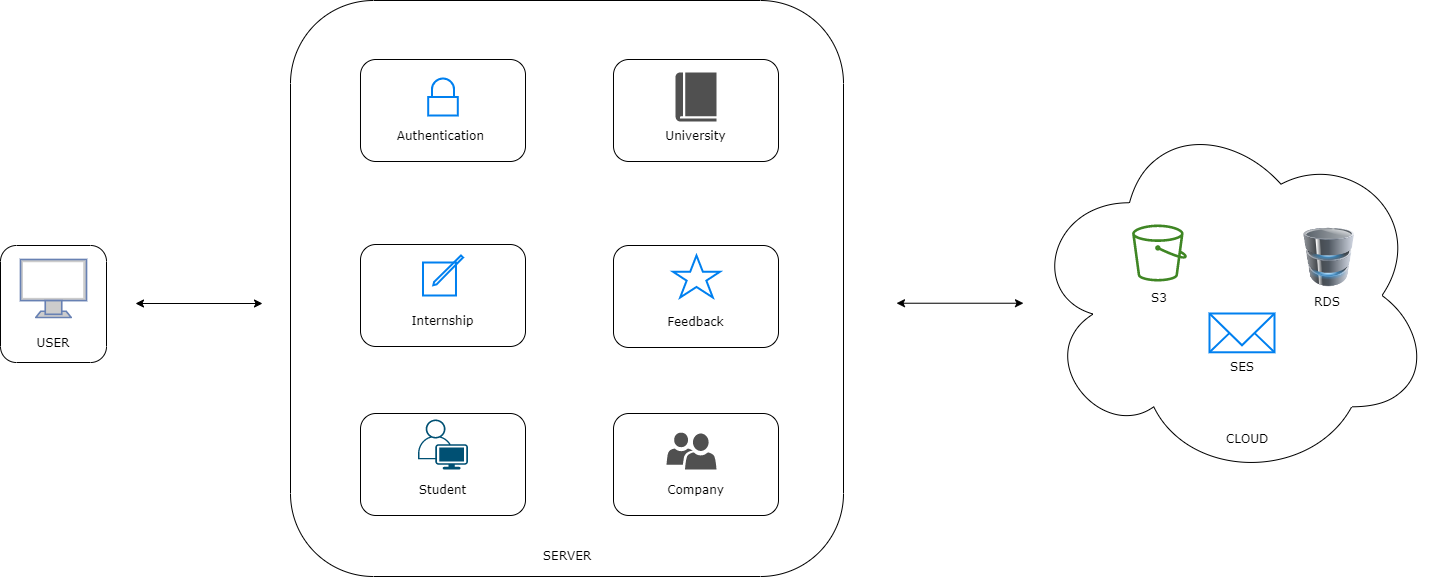
\includegraphics[scale=0.30]{Images/ImagesDD/overview.png}
    \caption{Overview diagram}
\end{figure}

The Students\&Companies (S\&C) platform is designed as a client-server application, where the term \textit{client} refers to the users of the system: students, companies, and universities. We have chosen a \textit{fat client} approach to provide a highly interactive, app-like experience, enabling responsive and rich functionality directly in the browser. This approach also reduces server load by offloading some processing to the client side, enhancing scalability.

Users interact with the system through a Single Page Application (SPA), a desktop web application that serves as the primary user interface for accessing platform features. The SPA allows for seamless navigation and interaction. By managing application state on the client side, the SPA minimizes page reloads, enhancing usability and responsiveness.

On the backend, we have followed a \textit{monolithic server} approach. This choice simplifies the overall system architecture by consolidating functionality into a single codebase, which can facilitate easier development, deployment, and maintenance. Although monolithic, the server is structured into multiple controllers and several business logic parts, each responsible for specific areas, such as authentication, internship management, profile handling, and recommendations. This modular organization within the monolith ensures that each component is cohesive and manageable while maintaining performance and consistency.

To support database, storage, and email services, we are using a cloud provider infrastructure. Specifically, we utilize Amazon Web Services (AWS) with Amazon RDS for the database, Amazon S3 for file storage, and Amazon SES for email notifications.


\newpage

\section{Component view}

\subsection{Client Components}
The principal component of the client side is the Web-App, which the user will interact with.

\subsection{Server Components}

In the server side, resides the principal components such as the controller used to manage the HTTP request sent by the user.

\begin{itemize}
\item \textbf{Internship}: Handles the logic related to managing internships, including creating, updating, and tracking internship opportunities. It allows administrators and companies to post internship positions and lets students apply, track, and view their application statuses.

\item \textbf{Student}: Manages all student-related data, including profile creation, academic details, and progress tracking. It allows students to update their profiles and view their application history, while administrators can monitor student progress and make updates as needed.

\item \textbf{Match}: Manages all the matches between the students and the companies' internship, finding matching between the suitable skills. Allows sending invitation to the student, and accepting those ones.

\item \textbf{Feedback}: Implements the system for collecting and managing feedback from students, companies, and administrators. This component allows participants to submit feedback on internship experiences, and administrators can review and analyze this feedback to improve the program.

\item \textbf{Company}: Responsible for managing company accounts and profiles, as well as facilitating company interactions with students and internships. It allows companies to create profiles, post internship opportunities, and review student applications, making the hiring and feedback process streamlined and accessible.

\item \textbf{University}: Responsible for managing university interaction with the platform. Such as tracking students' internship, reading their feedback and leaving a feedback about the platform.


\item \textbf{Authentication}:
The Authentication handles all processes related to user authentication, such as logging in, logging out, session validation, and password management.
\end{itemize}

\subsection{Data Component}

We use a relational database hosted on AWS to securely manage and organize structured data for the application. AWS’s managed RDS service offers high availability, automated backups, and scalability, ensuring reliable data storage and quick access for all server components. This setup allows us to maintain relational integrity, enforce data consistency, and easily scale as our data requirements grow.


\begin{figure}[!ht]
    \centering
    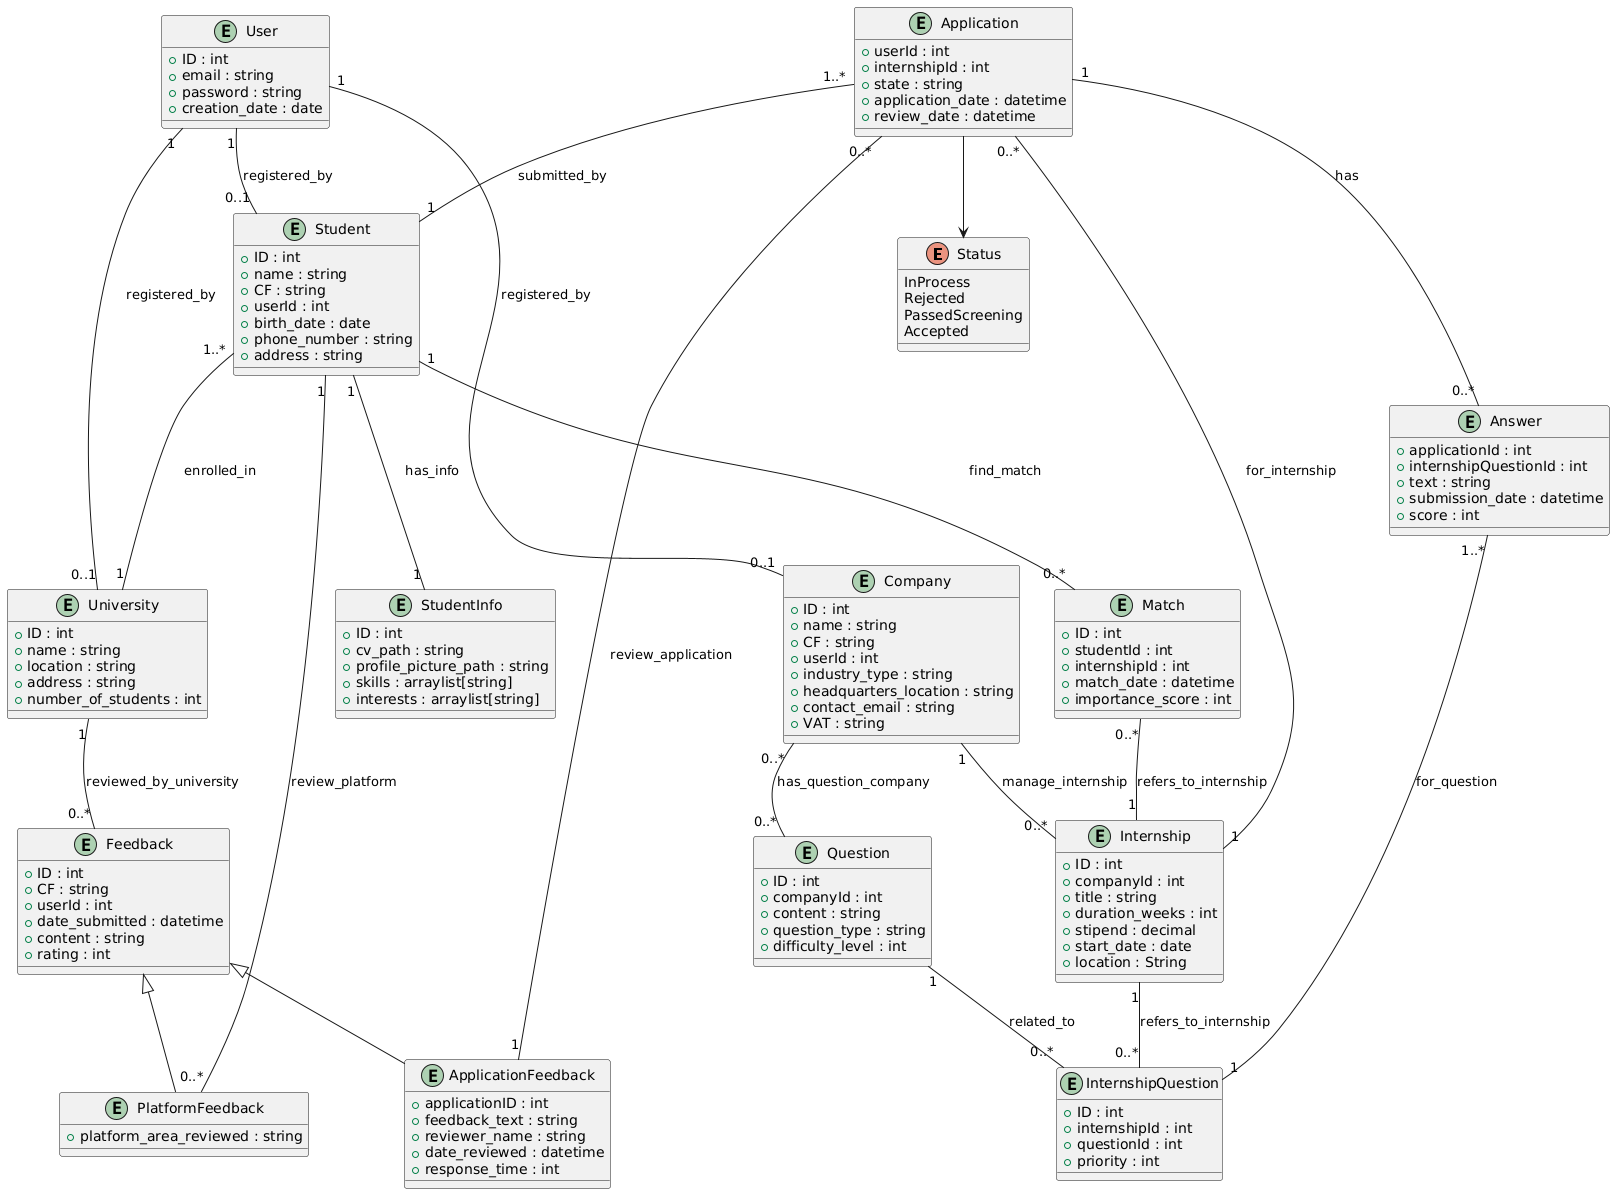
\includegraphics[scale=0.30]{Images/ImagesDD/class_diagram.png}
    \caption{Class diagram referring to the data components}
\end{figure}


\section{Deployment view}

The frontend is a SPA implemented with the React framework. The website can be visited from any modern web browser, such as Google Chrome, Mozilla Firefox or Microsoft Edge. \\ \\
Clients can be any desktop device that can run the previous browsers, such as computers with Windows, Linux or macOS.
The website is served by a CDN like Amazon CloudFront.
Using a CDN greatly enhances performance by caching static assets on globally distributed servers, ensuring users access content from locations closest to them for faster load times and reduced latency. \\ \\
The backend of the platform is powered by an ASP.NET Core server, deployed within a Kubernetes cluster that orchestrates and manages the containerized environment. This setup ensures that the backend is scalable, resilient, and highly available, with Kubernetes automating the deployment, scaling, and management of application pods. NGINX is used within the cluster as an Ingress Controller, handling incoming traffic, SSL termination, and advanced routing rules. Kubernetes performs horizontal scaling by automatically deploying new pods during traffic surges to maintain seamless performance.\\ \\
The ASP.NET Core application communicates with AWS services like RDS for database and S3 for storage. Continuous integration and deployment pipelines facilitate automated updates, pushing new Docker images to the cluster and enabling rolling updates with minimal downtime.\\ \\
This integration of Kubernetes and NGINX ensures that the backend infrastructure is robust and adaptable, capable of handling large volumes of requests while providing efficient load distribution and reliability.

\begin{figure}[!ht]
    \centering
    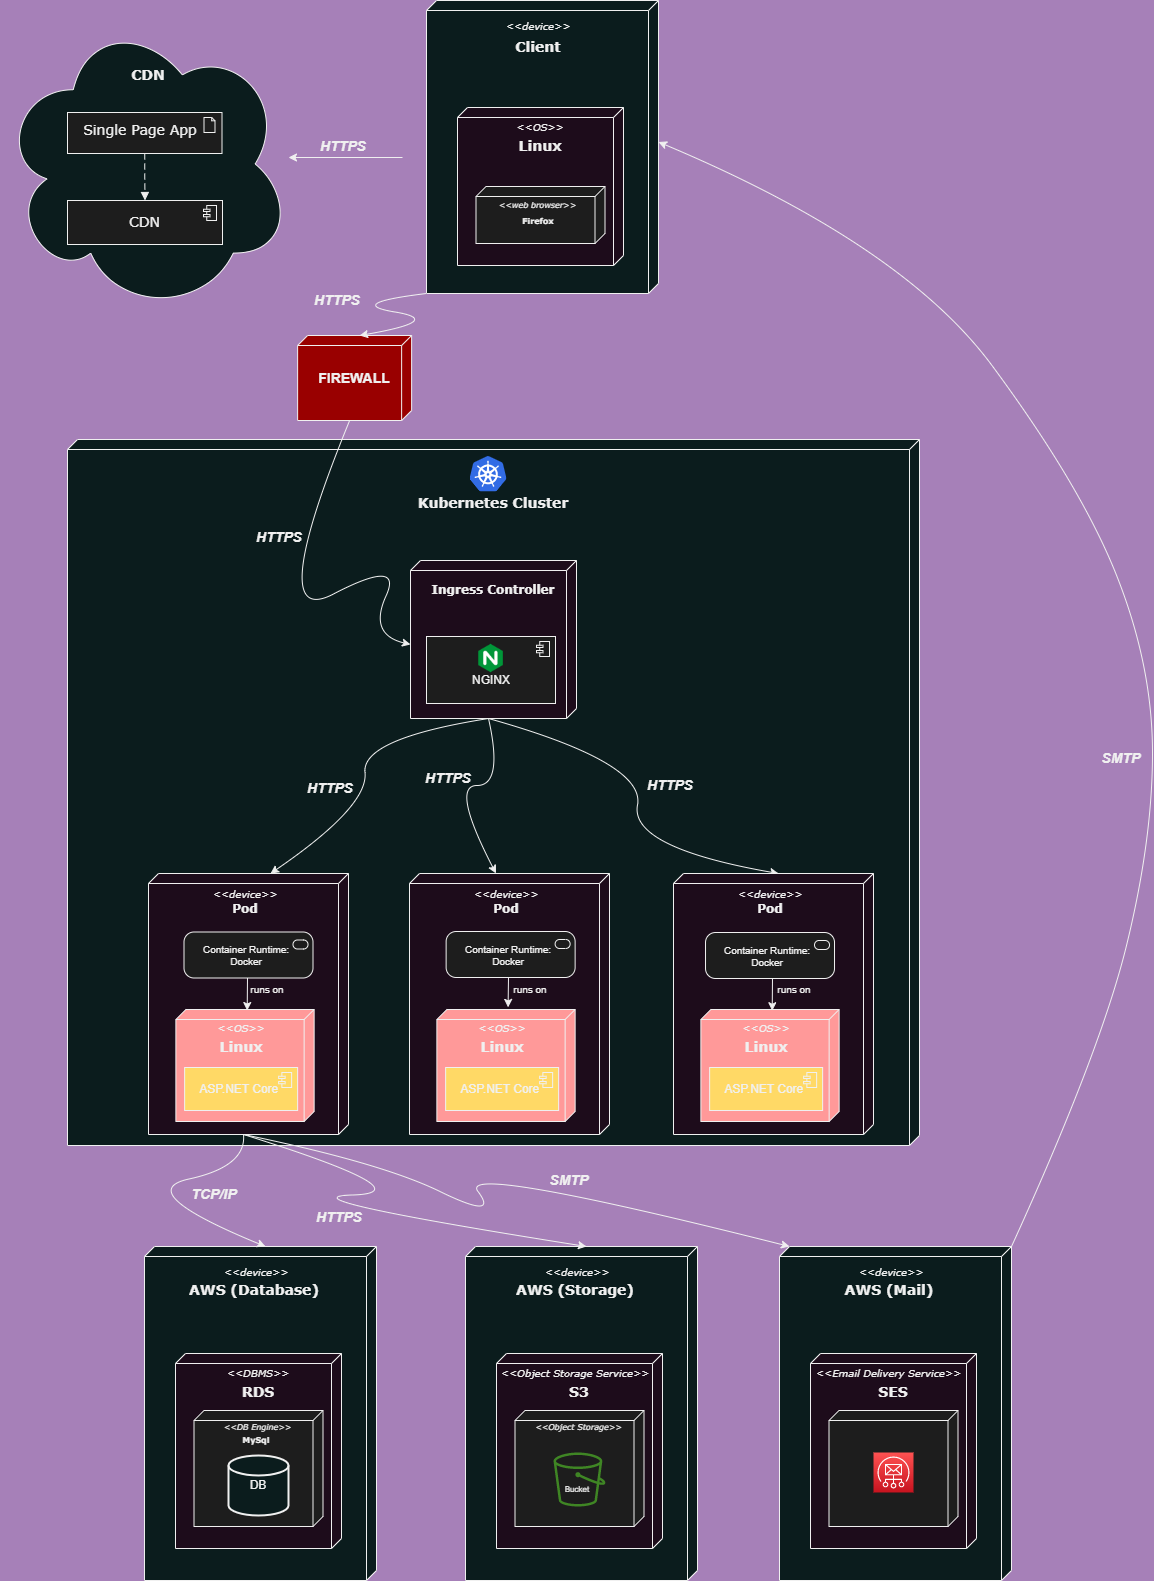
\includegraphics[scale=0.30]{Images/ImagesDD/deployment.png}
    \caption{Deployment diagram}
\end{figure}

\newpage


\section{Runtime view}
The following sequence diagrams illustrate the interactions between system components. 

Each diagram corresponds to and represents the implementation of its respective use case, as described in the RASD document, in the same order.

In each sequence diagram it is omitted the part specified in the diagram 0.1, that illustrates the case of unauthorized access and the tentative to gain a new valid authentication token. 

The following function (2.2) for simplicity is represented in another diagram, but it is meant to be intended as an action that happens before all the other diagrams.
\vspace{5mm}

\begin{figure}[ht!]
    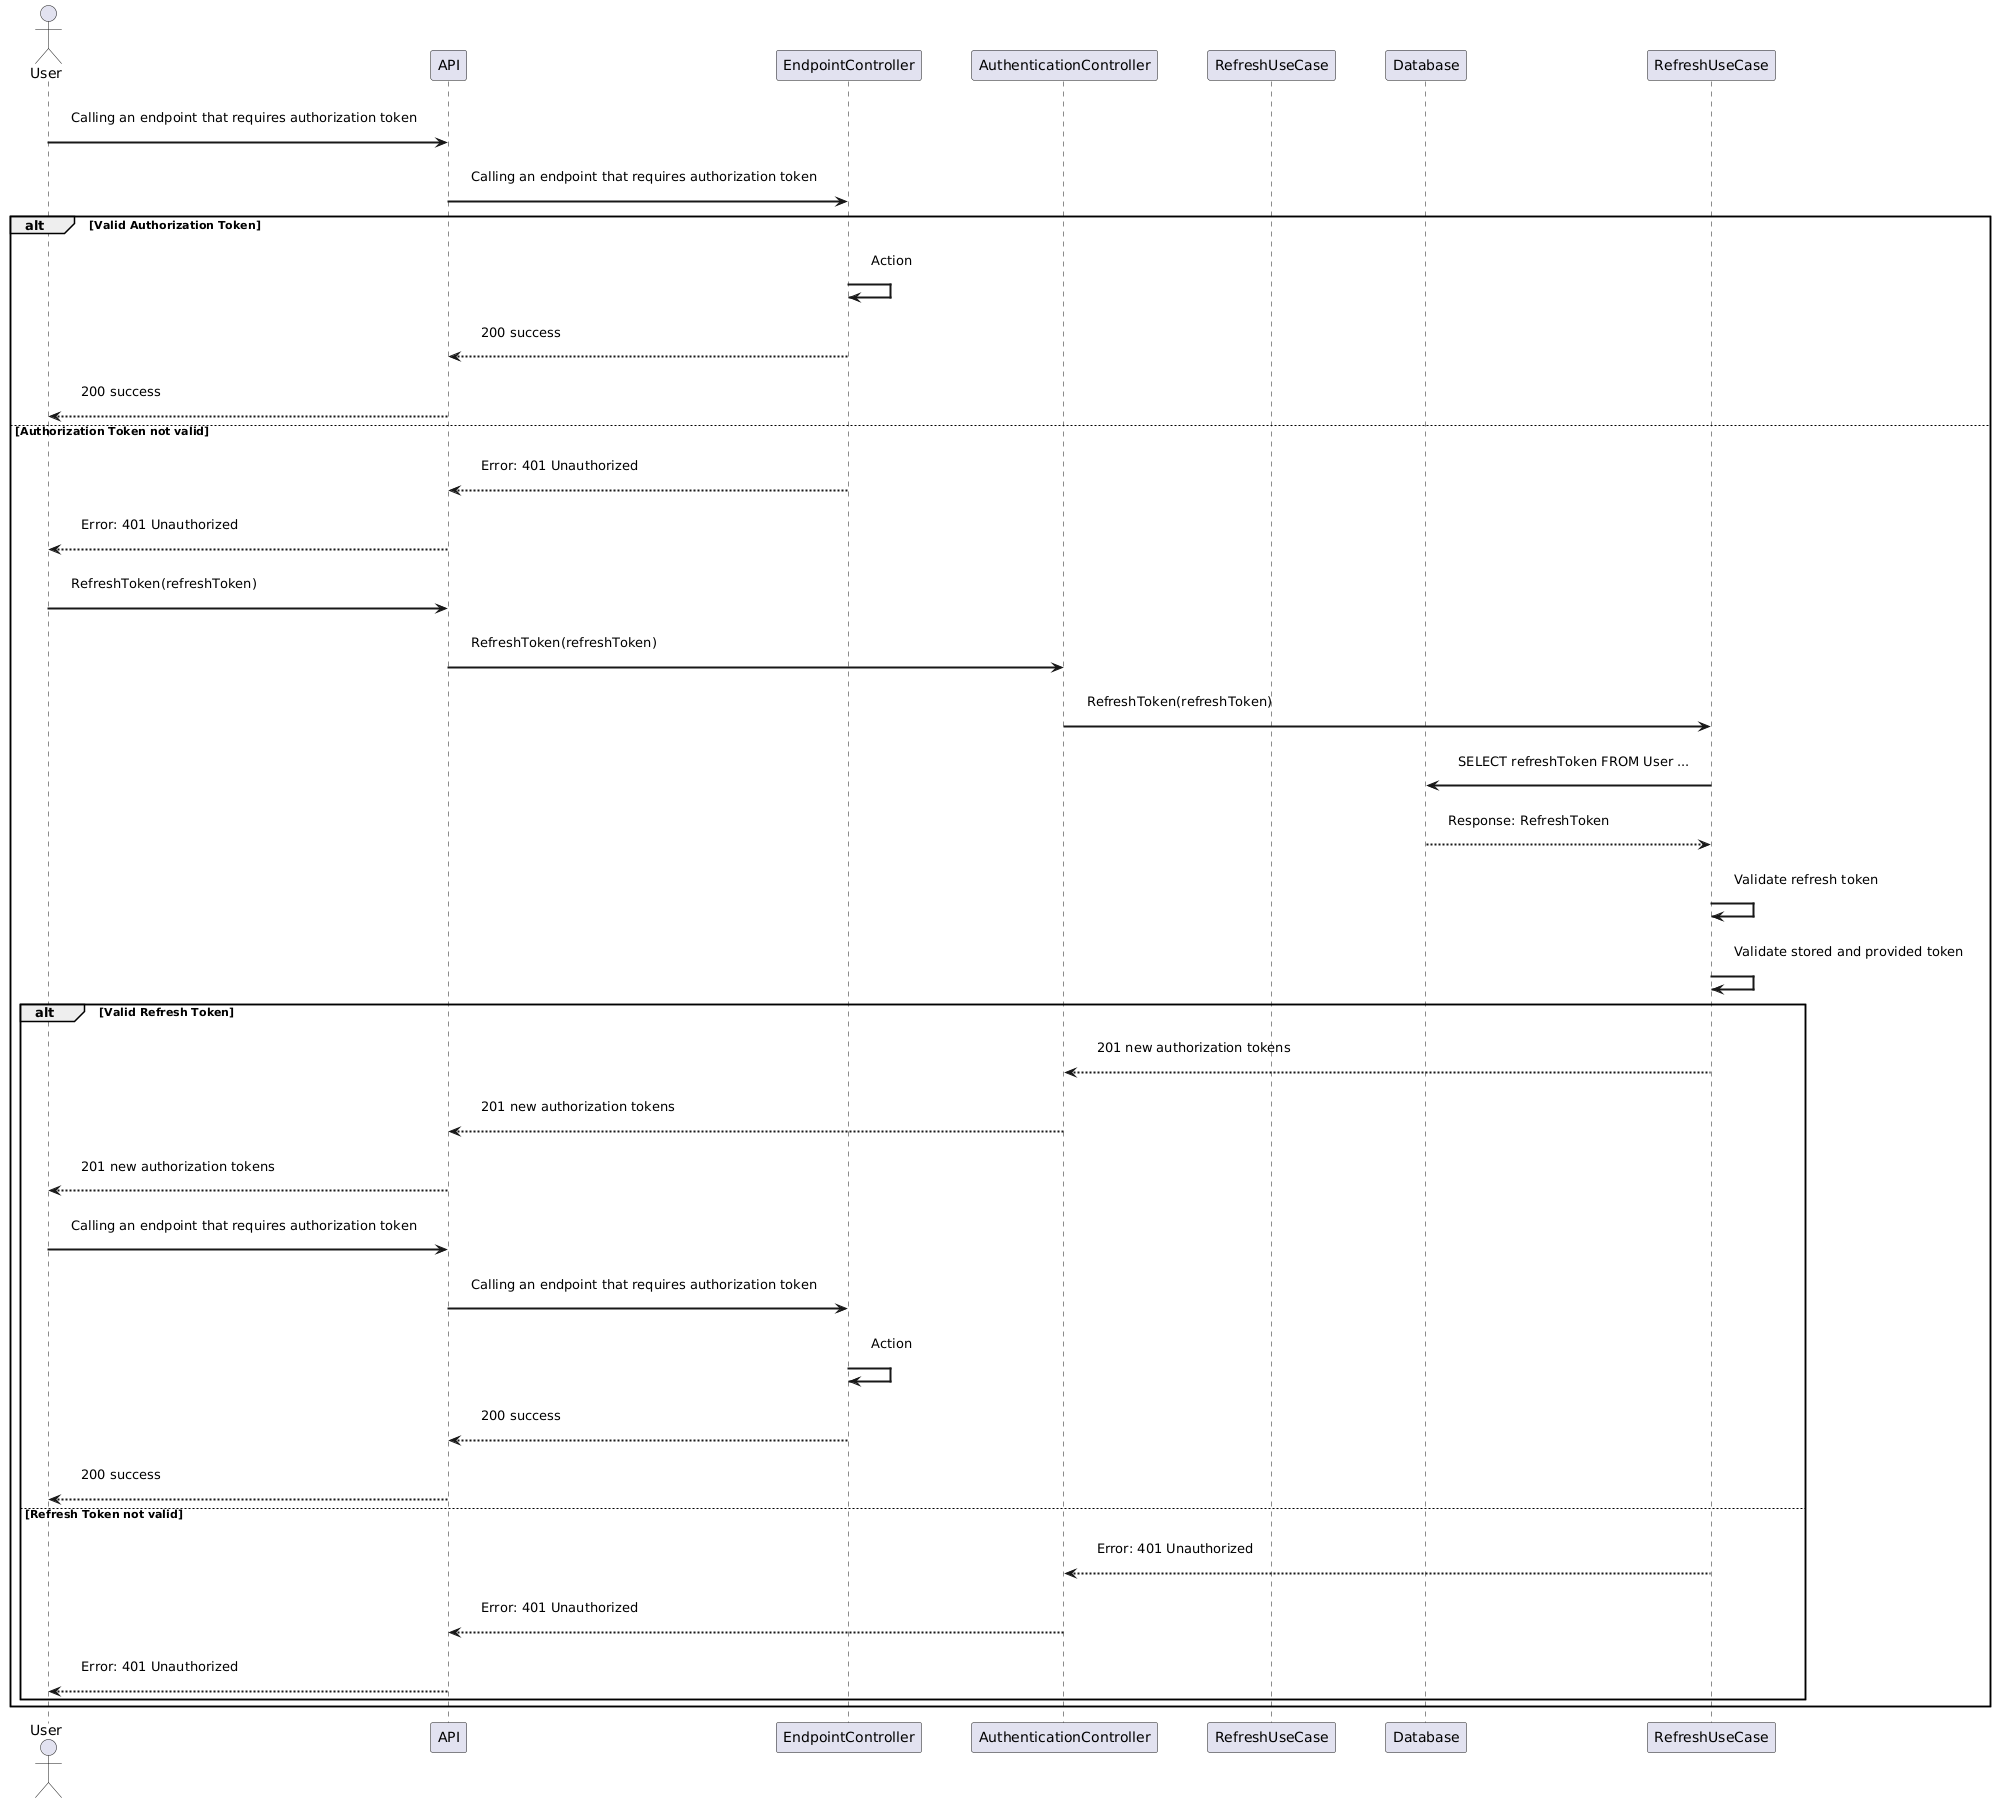
\includegraphics[scale=0.29]{Images/ImagesSequenceDiagram/AuthSequenceFlow.png}
    \caption{Sequence diagram 0.1 : Authorization Flow}
\end{figure}

\begin{figure}[ht!]
    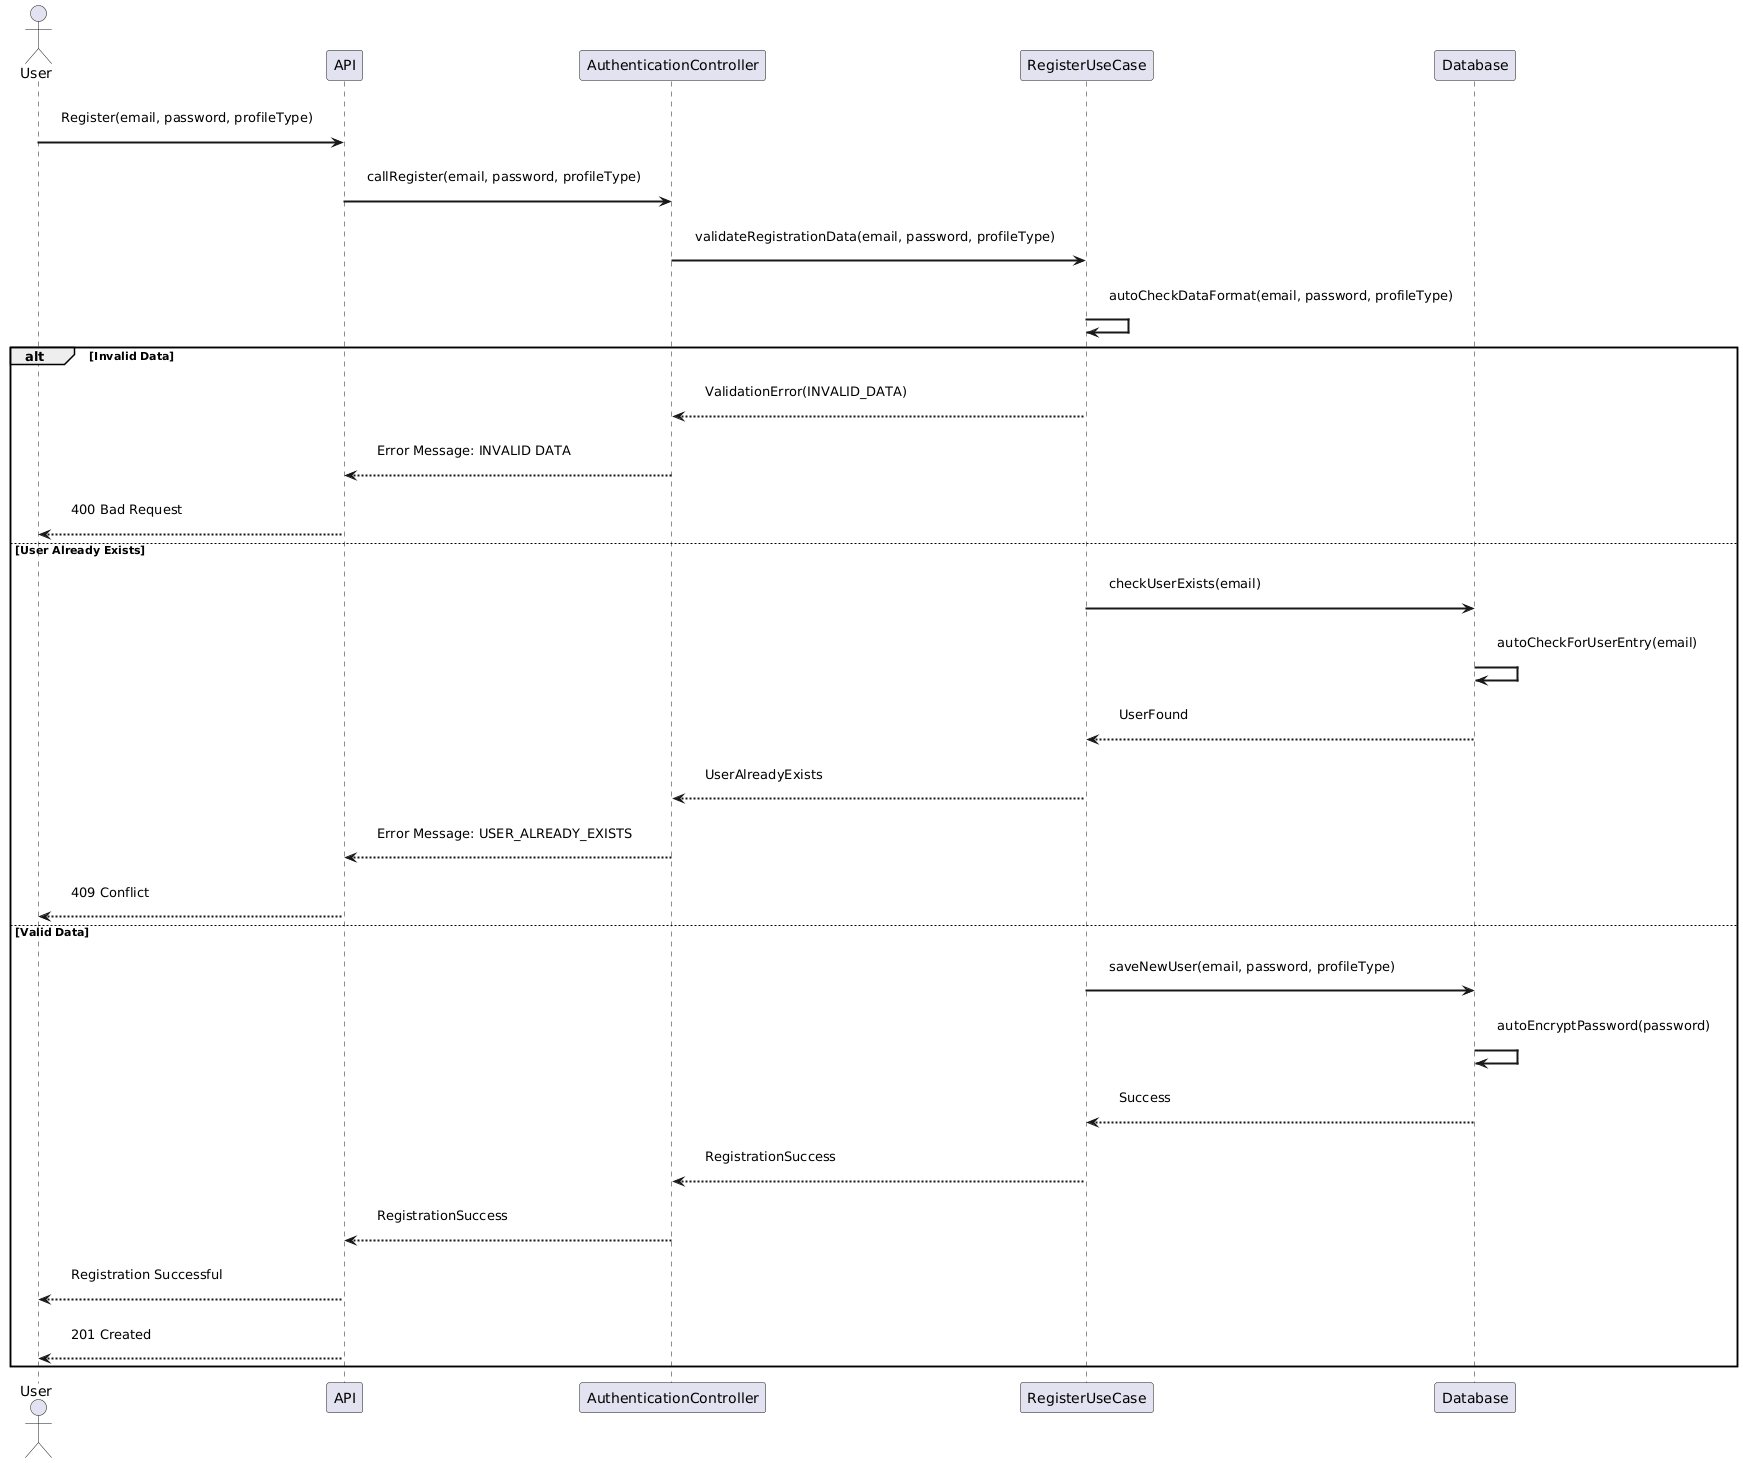
\includegraphics[scale=0.29]{Images/ImagesSequenceDiagram/RegisterAuthentication.png}
    \caption{User (Student, Company or University) Registration}
\end{figure}

\newpage

\begin{figure}[ht!]
    \centering
    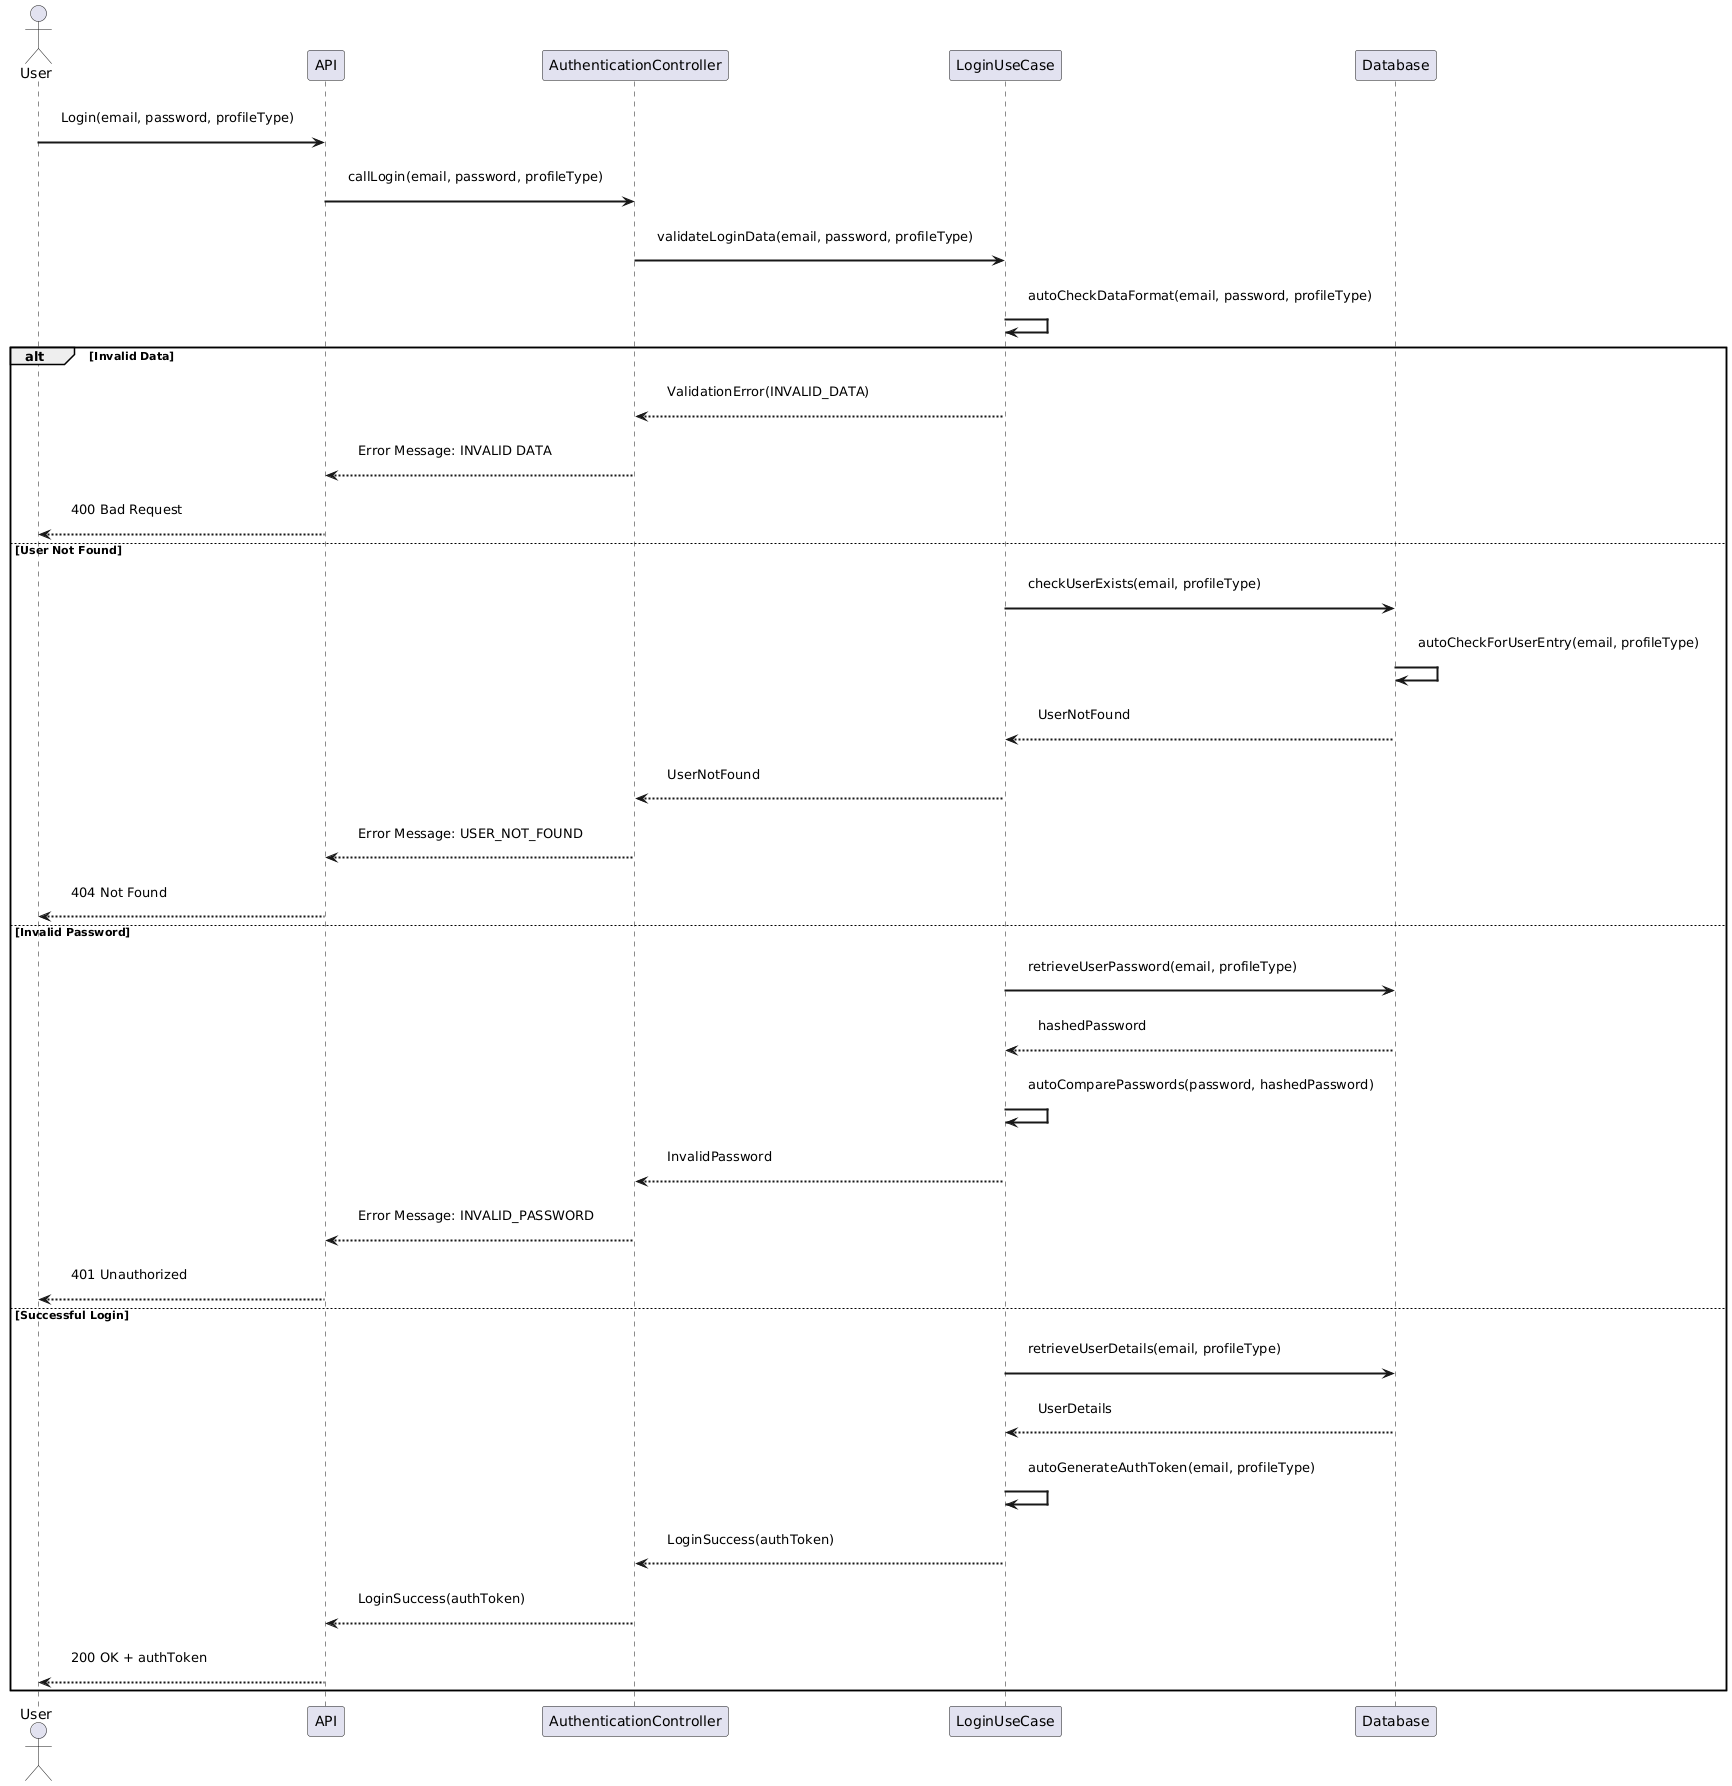
\includegraphics[scale=0.27]{Images/ImagesSequenceDiagram/LoginAuthentication.png}
    \caption{User (Student, Company or University) Login}
\end{figure}

\newpage

\begin{figure}[ht!]
    \centering
    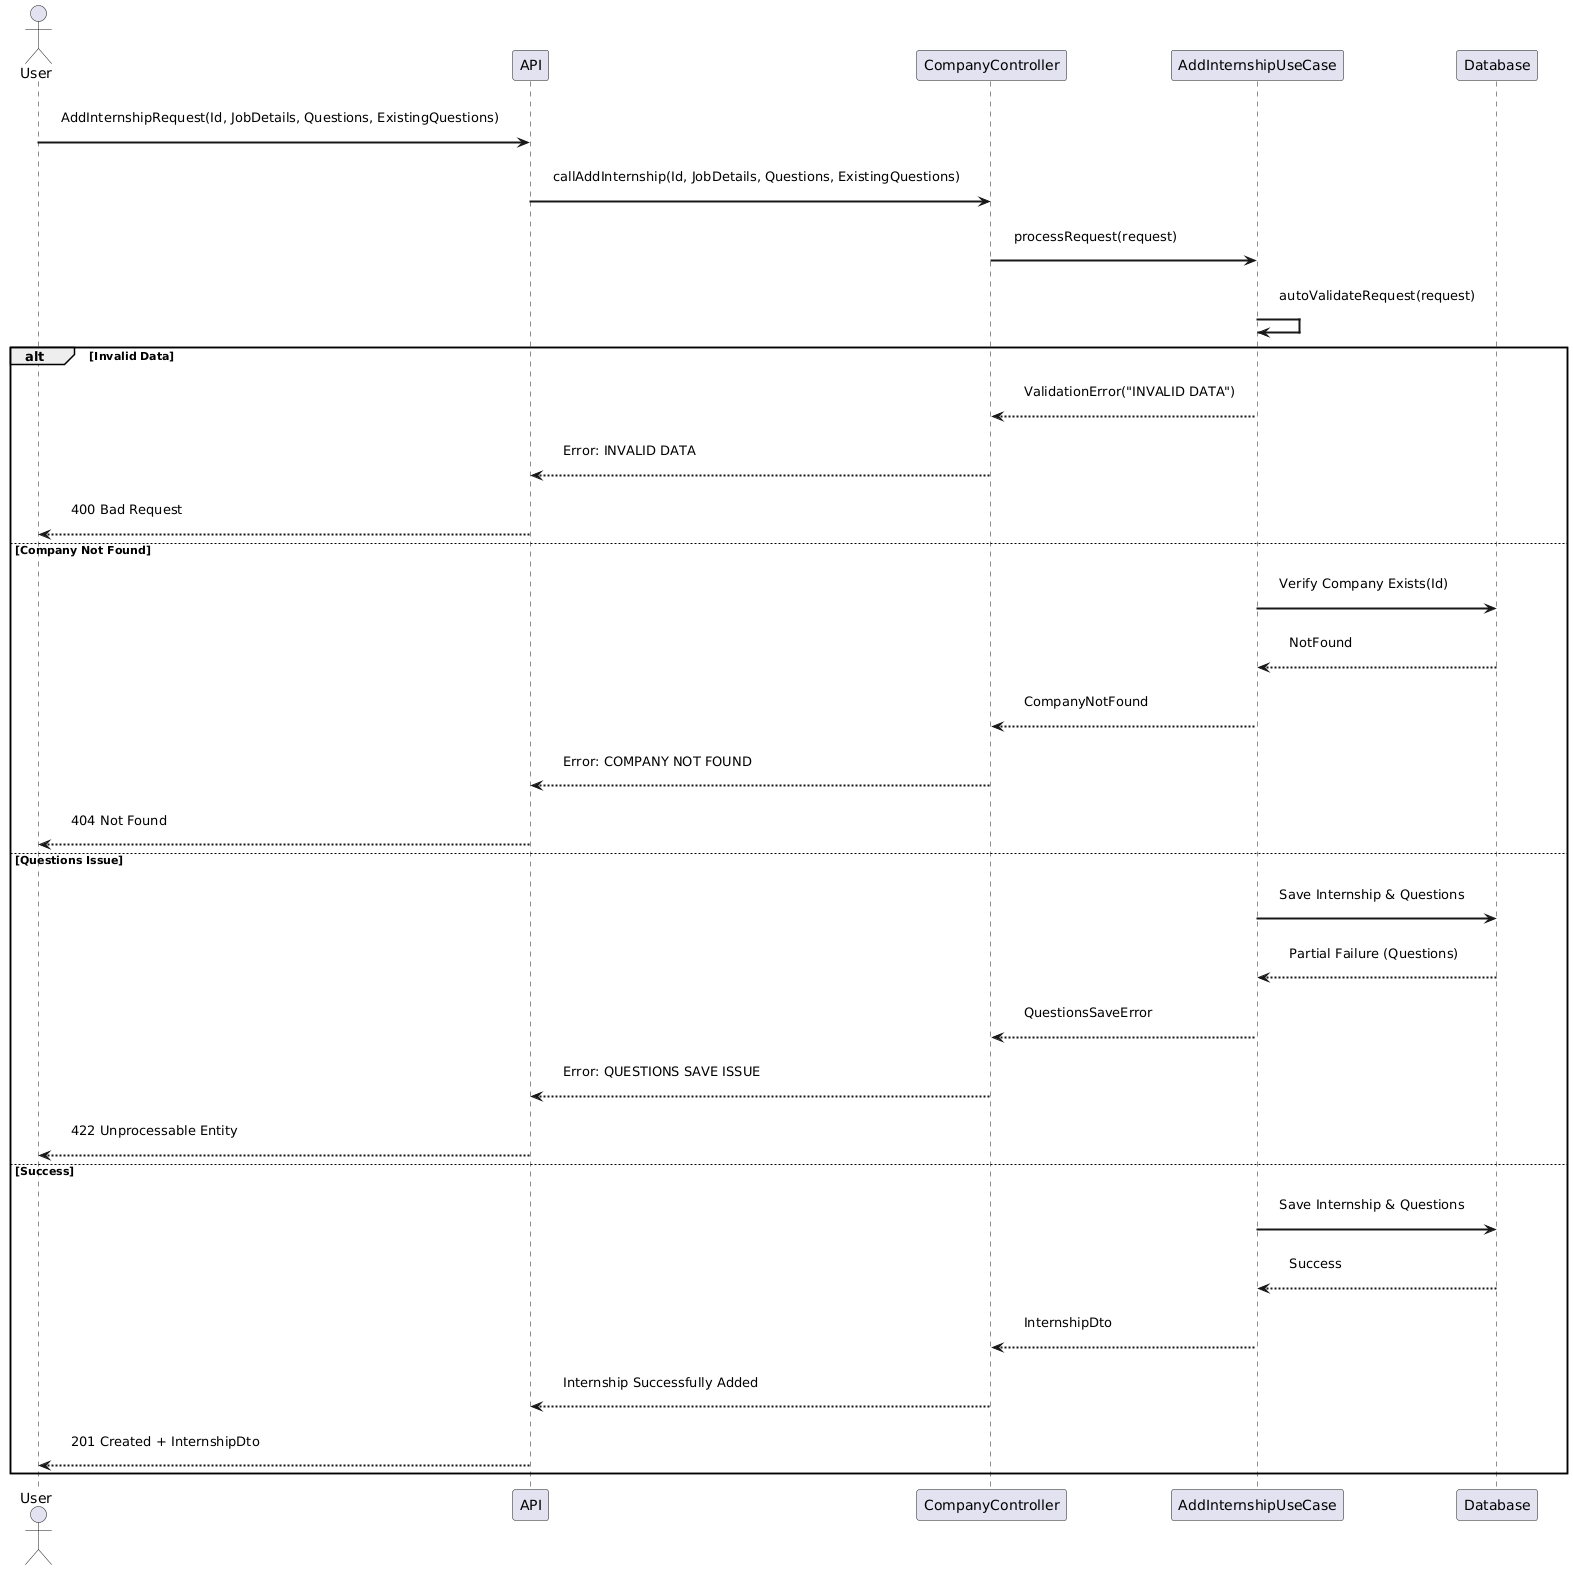
\includegraphics[scale=0.3]{Images/ImagesSequenceDiagram/InternshipCreation.png}
    \caption{Internship post creation}
\end{figure}

\newpage

\begin{figure}[ht!]
    \centering
    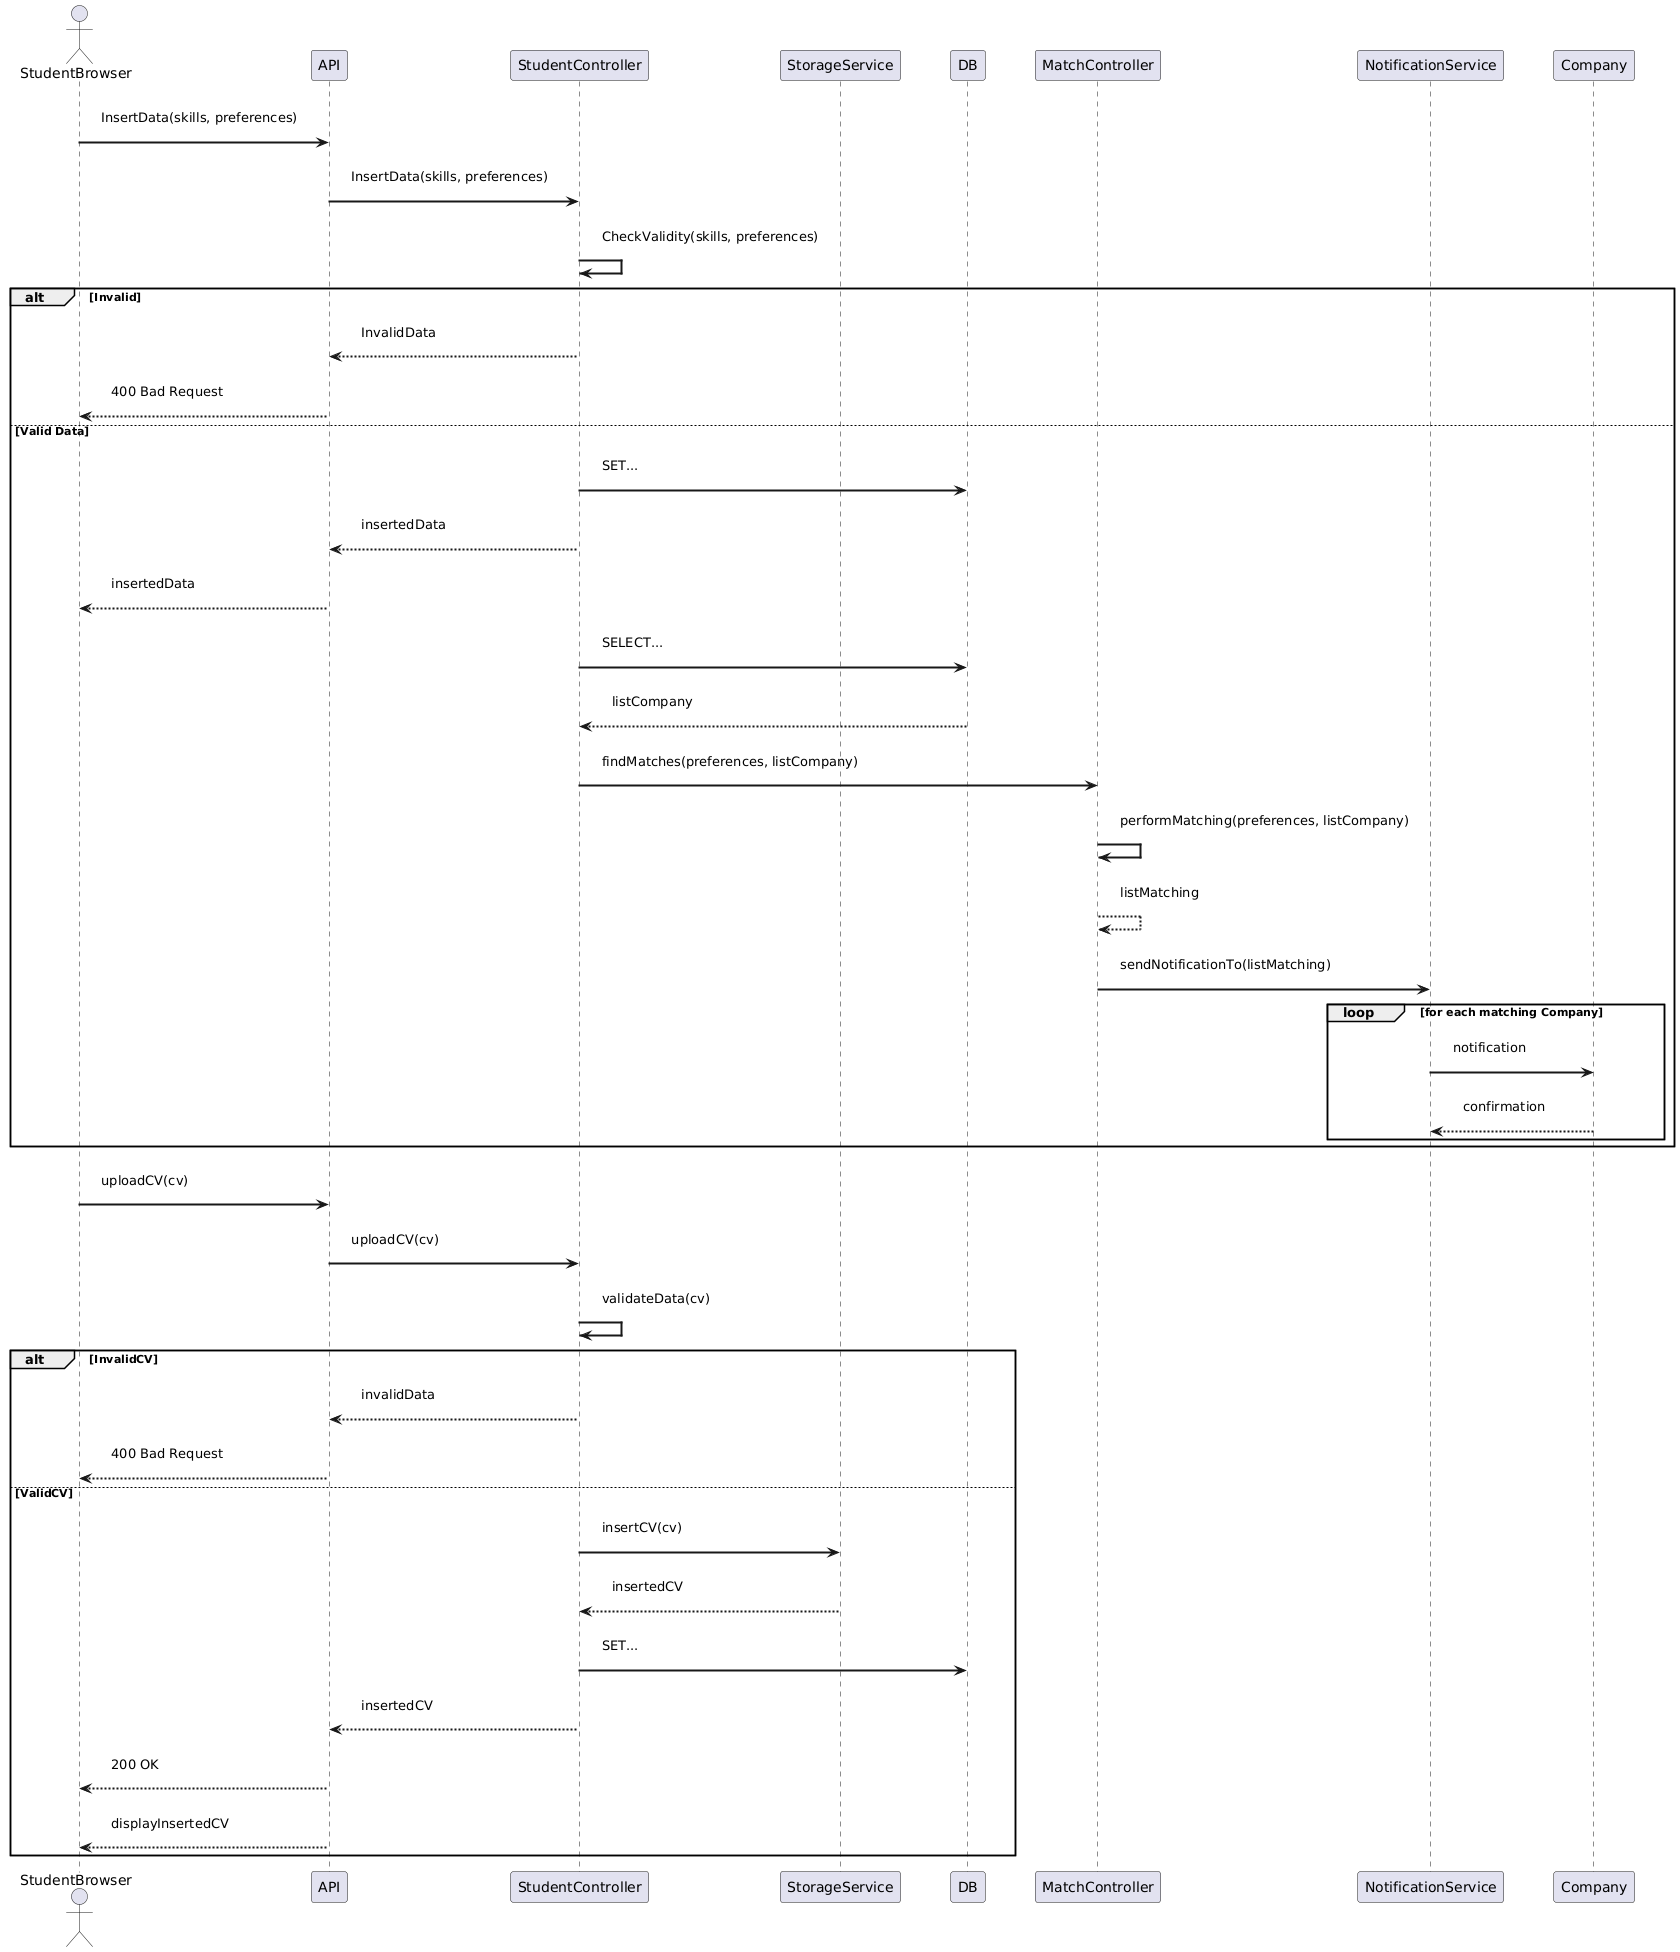
\includegraphics[scale=0.28]{Images/ImagesSequenceDiagram/StudentUploadCV.png}
    \caption{Student inserts CV and data}
\end{figure}

\newpage

\begin{figure}[ht!]
    \centering
    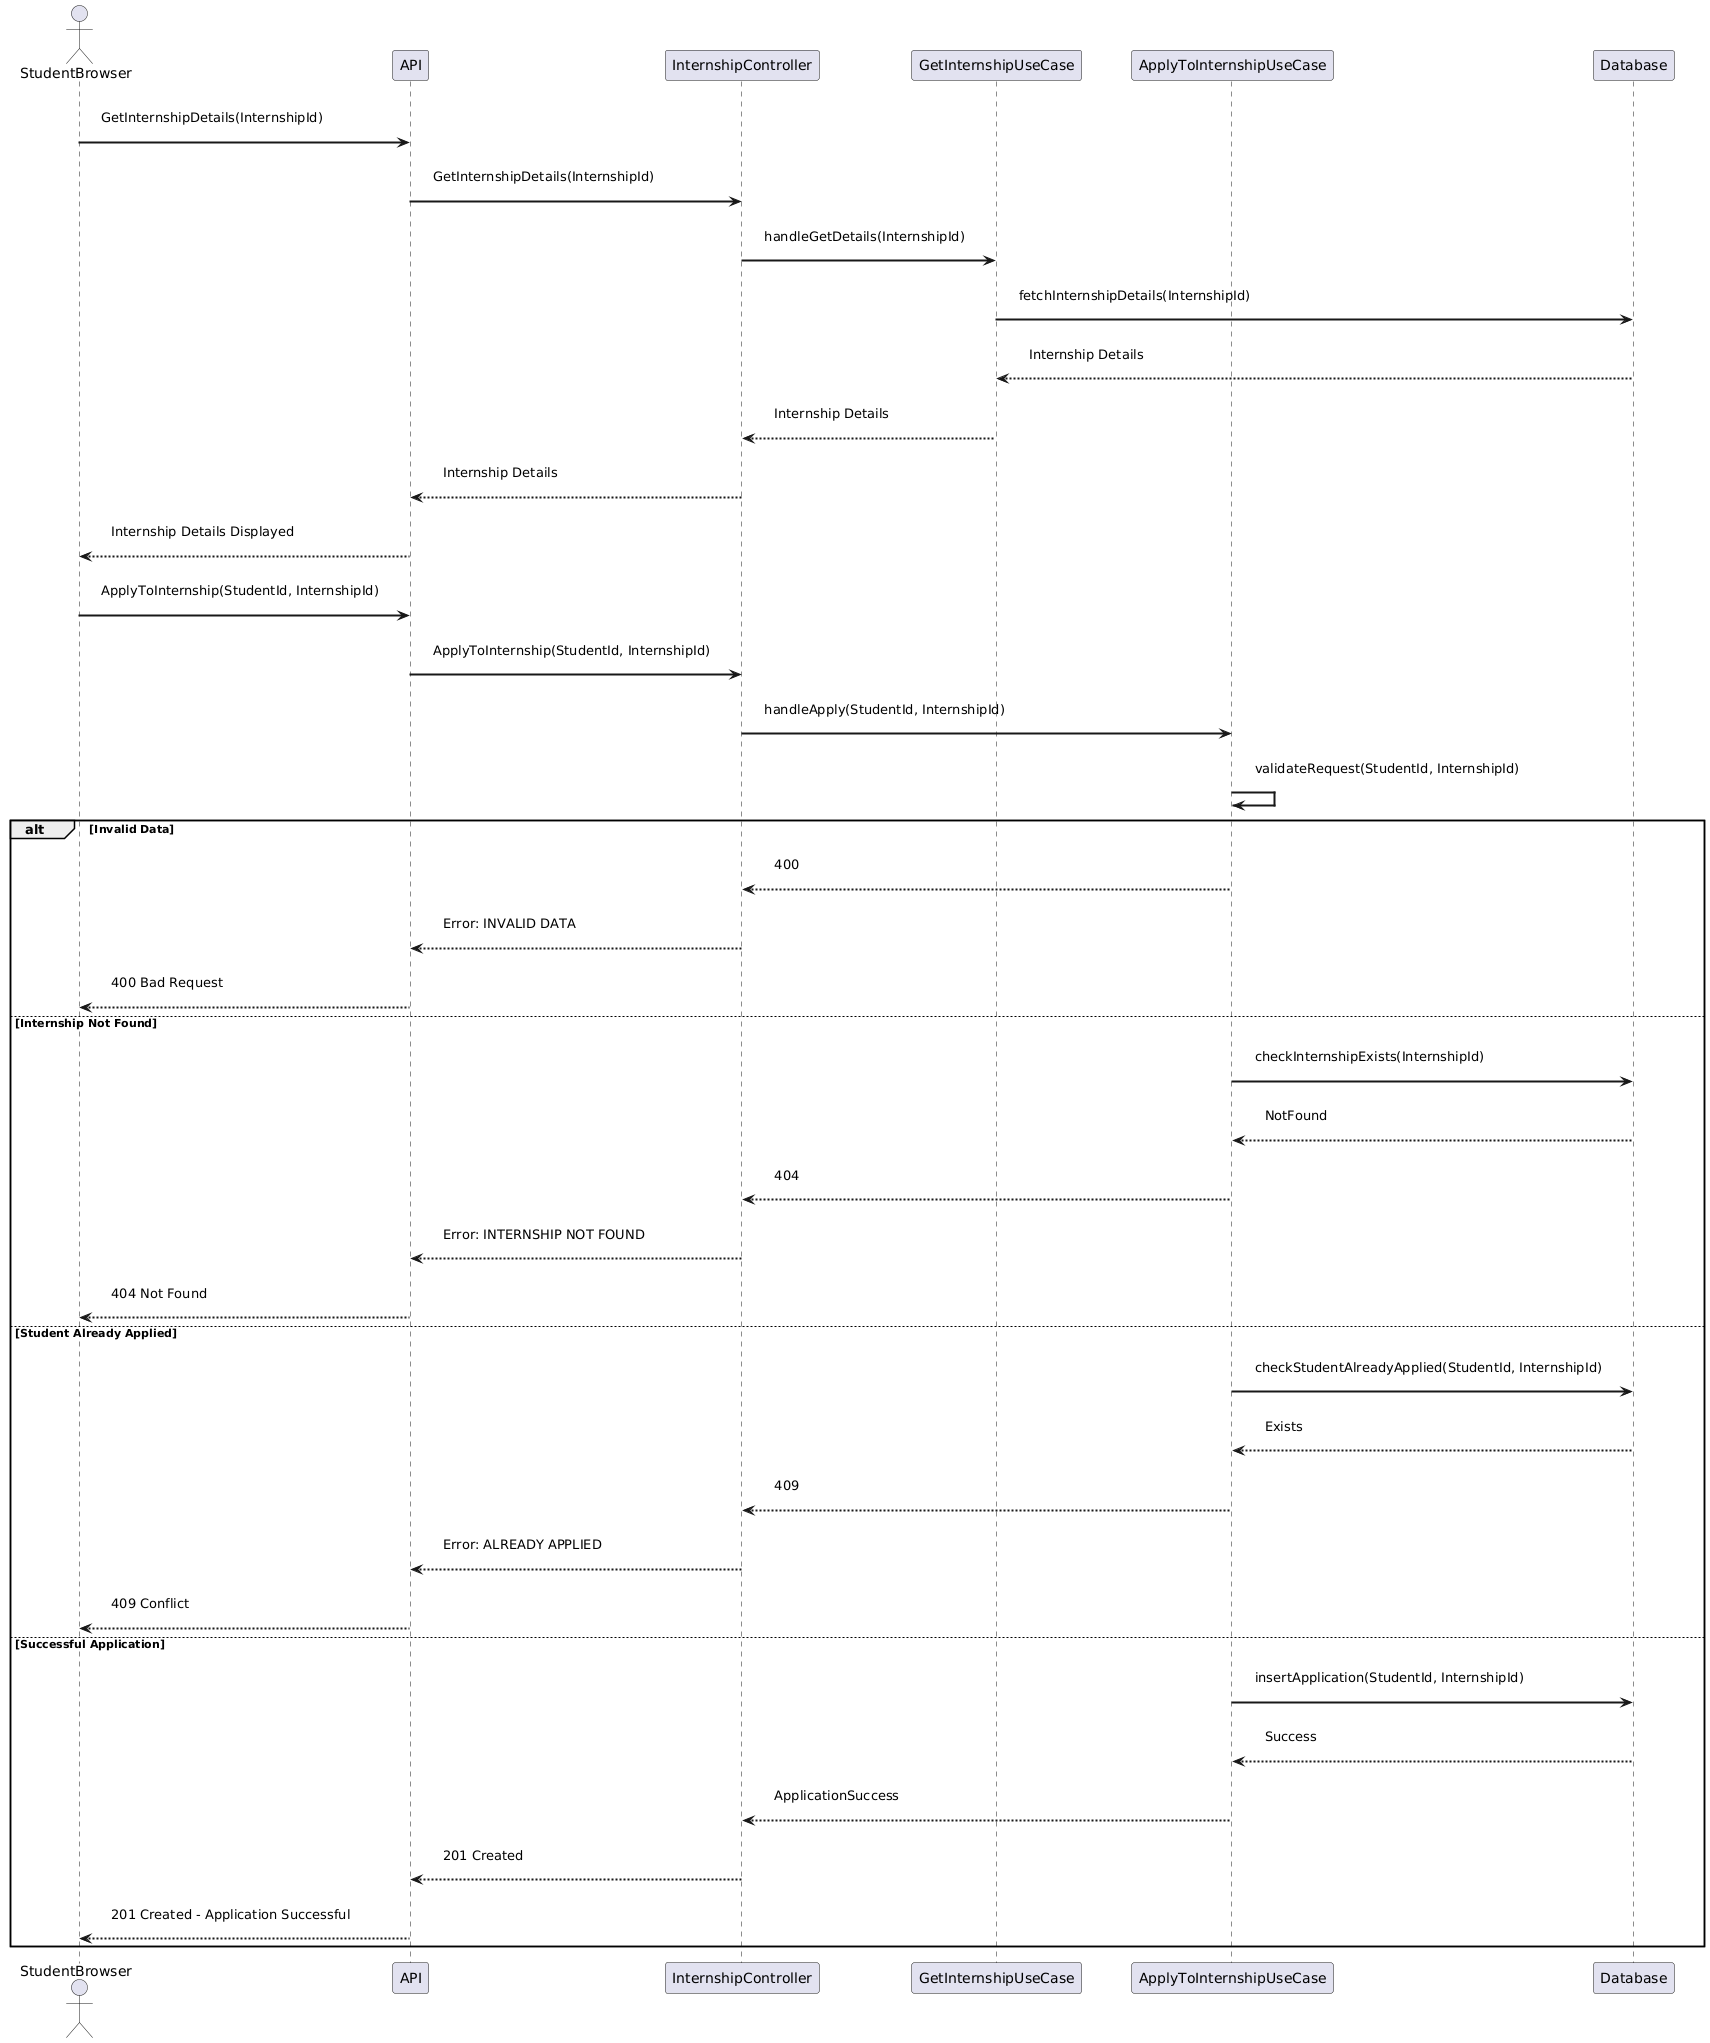
\includegraphics[scale=0.28]{Images/ImagesSequenceDiagram/StudentSubmitApplication.png}
    \caption{Student submit an application to an internship}
\end{figure}

\newpage

\begin{figure}[ht!]
    \centering
    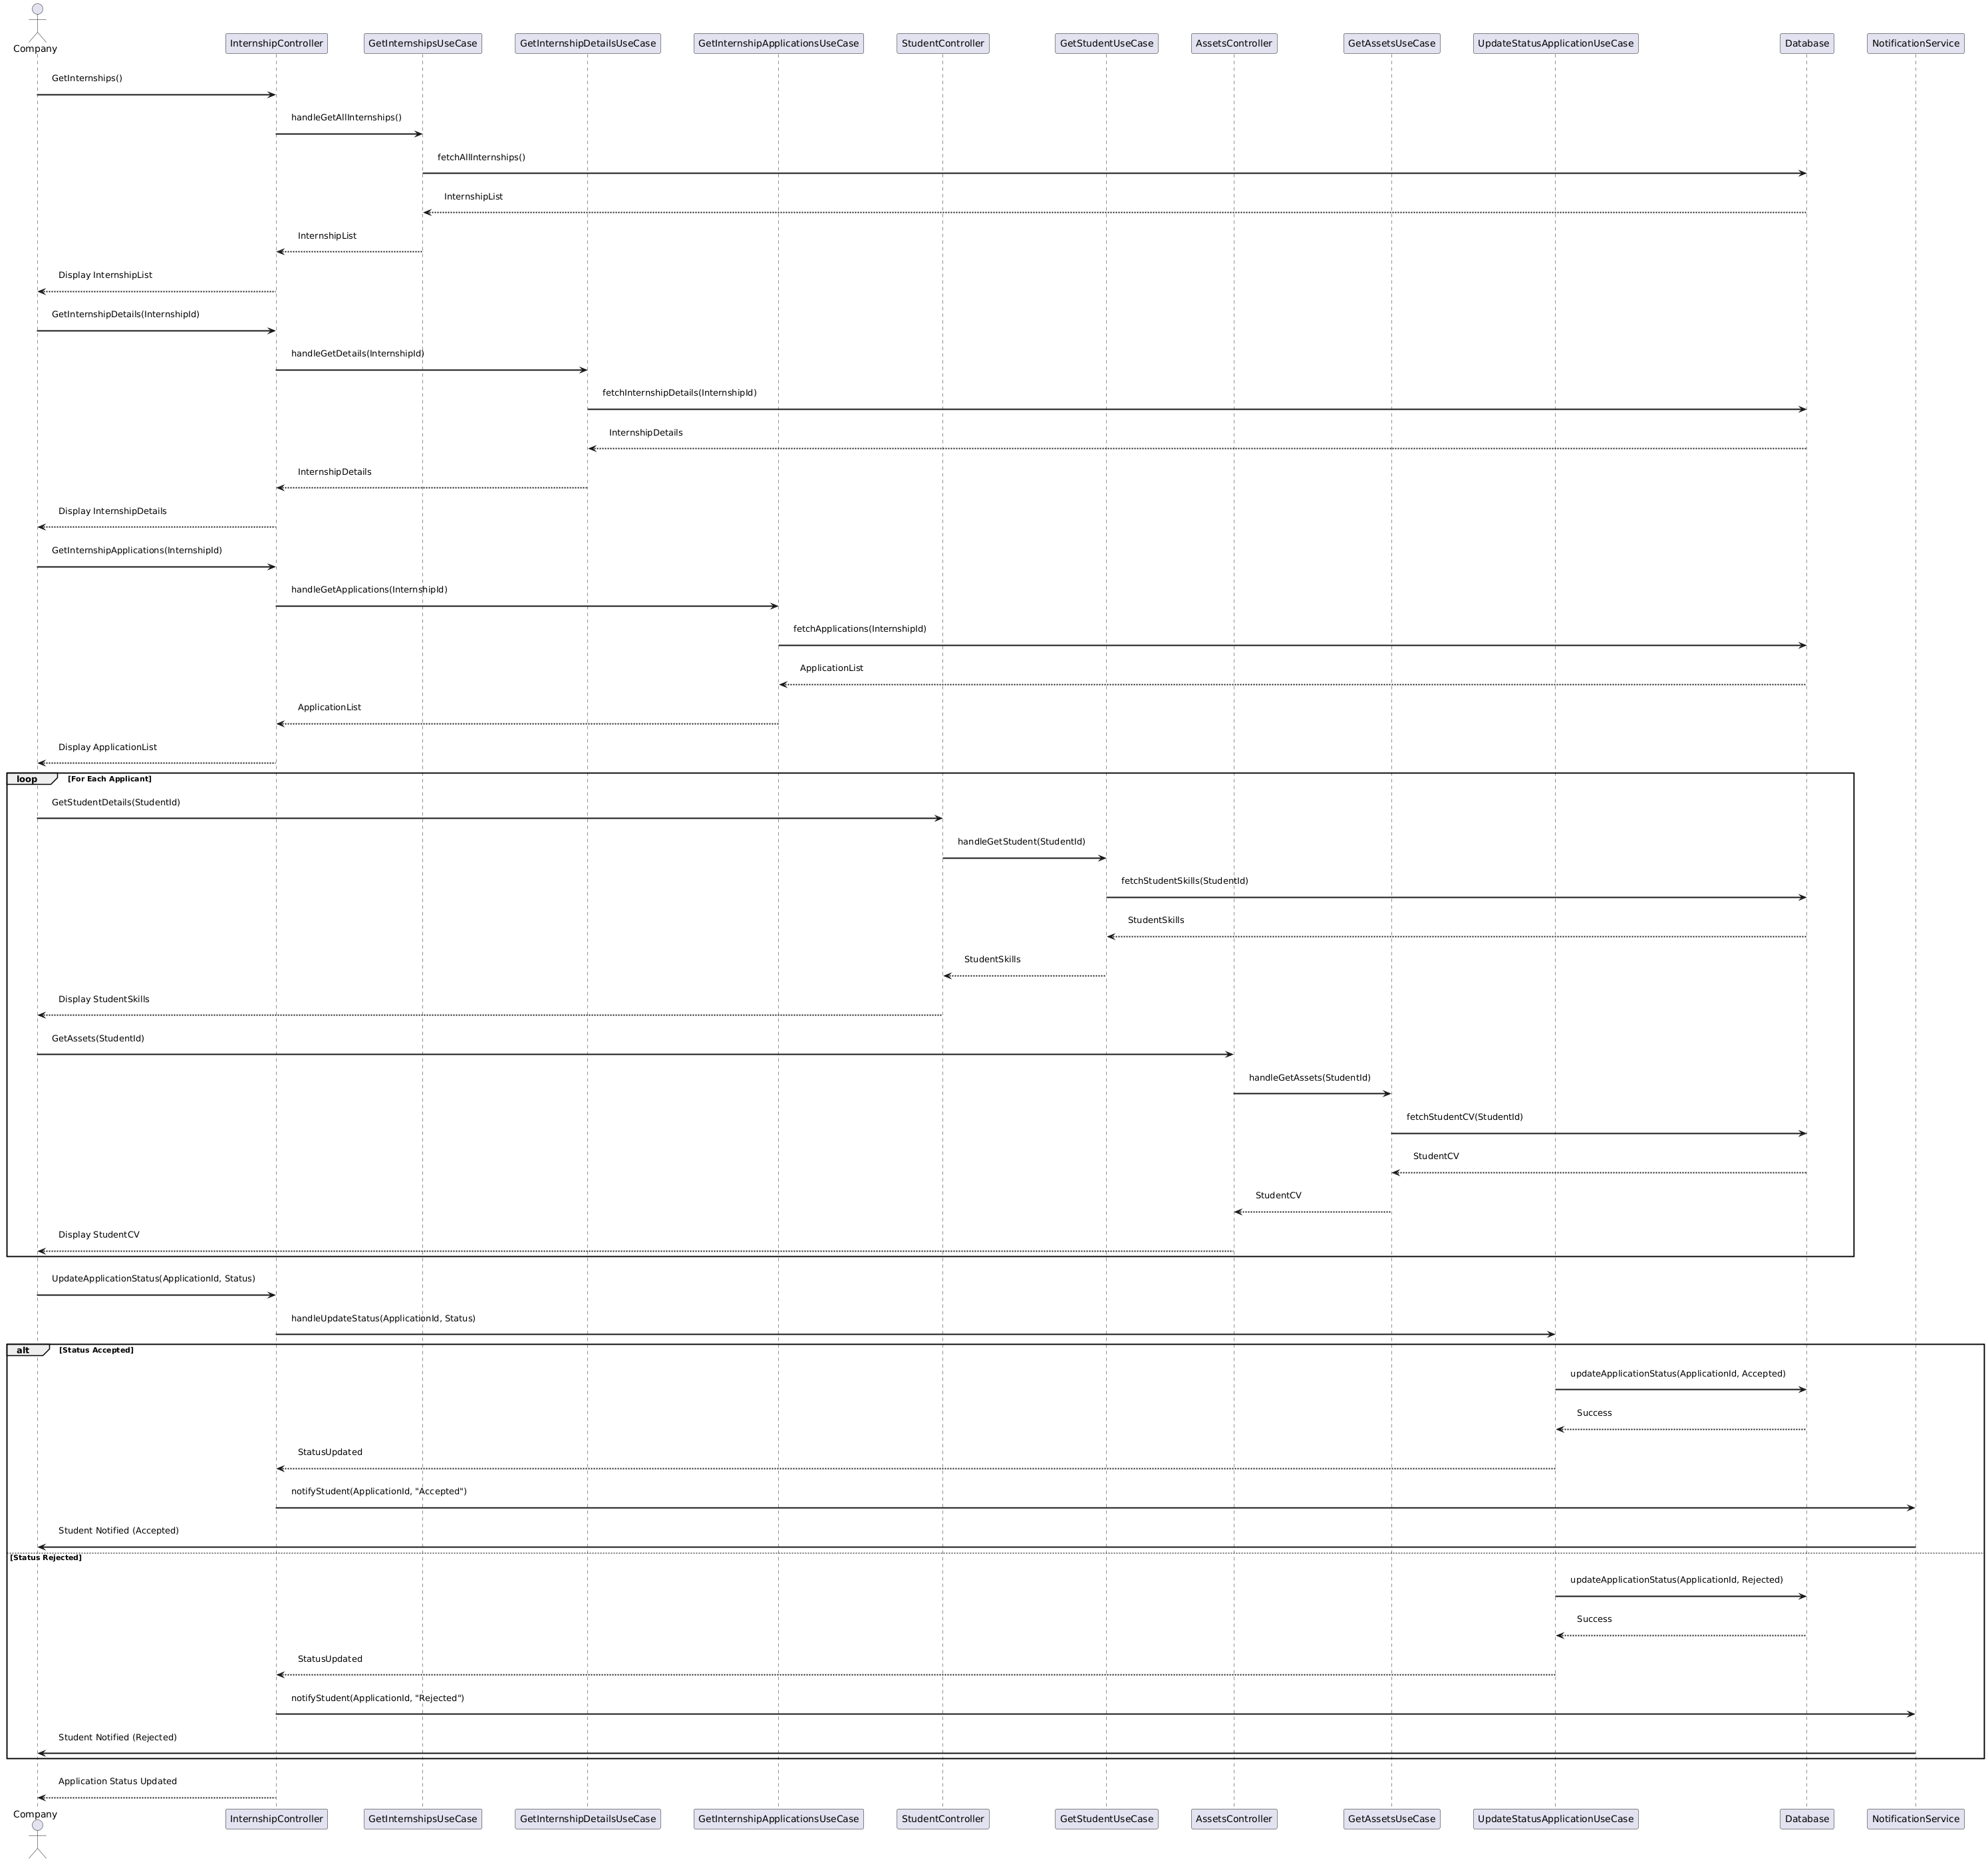
\includegraphics[scale=0.15]{Images/ImagesSequenceDiagram/CompanyManagesIncomeApplications.png}
    \caption{Company management of internship applications}
\end{figure}

\newpage

\begin{figure}[ht!]
    \centering
    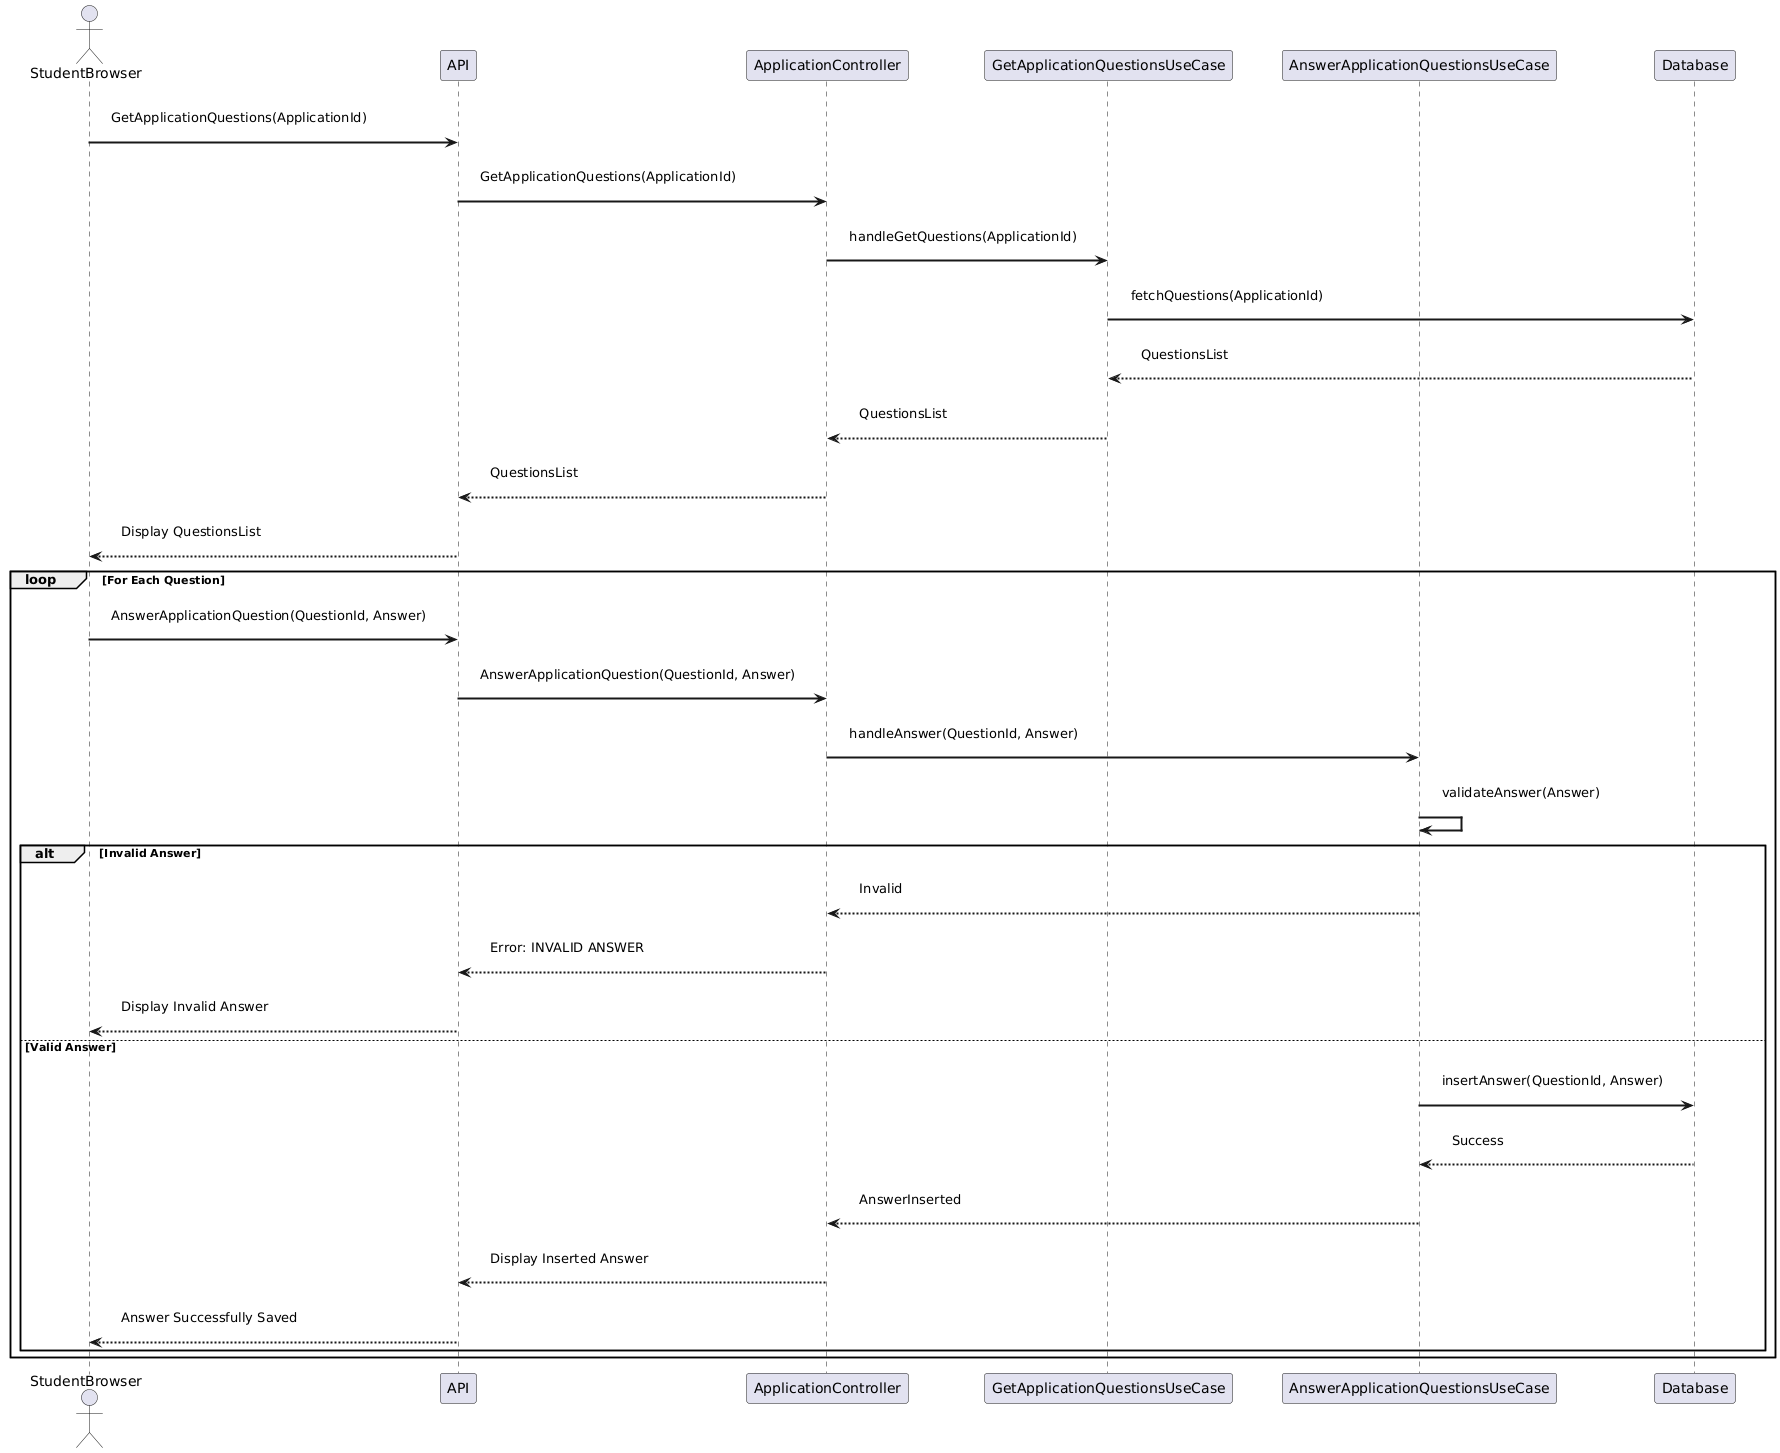
\includegraphics[scale=0.28]{Images/ImagesSequenceDiagram/StudentAnswereQuestions.png}
    \caption{Student answers questions}
\end{figure}

\newpage

\begin{figure}[ht!]
    \centering
    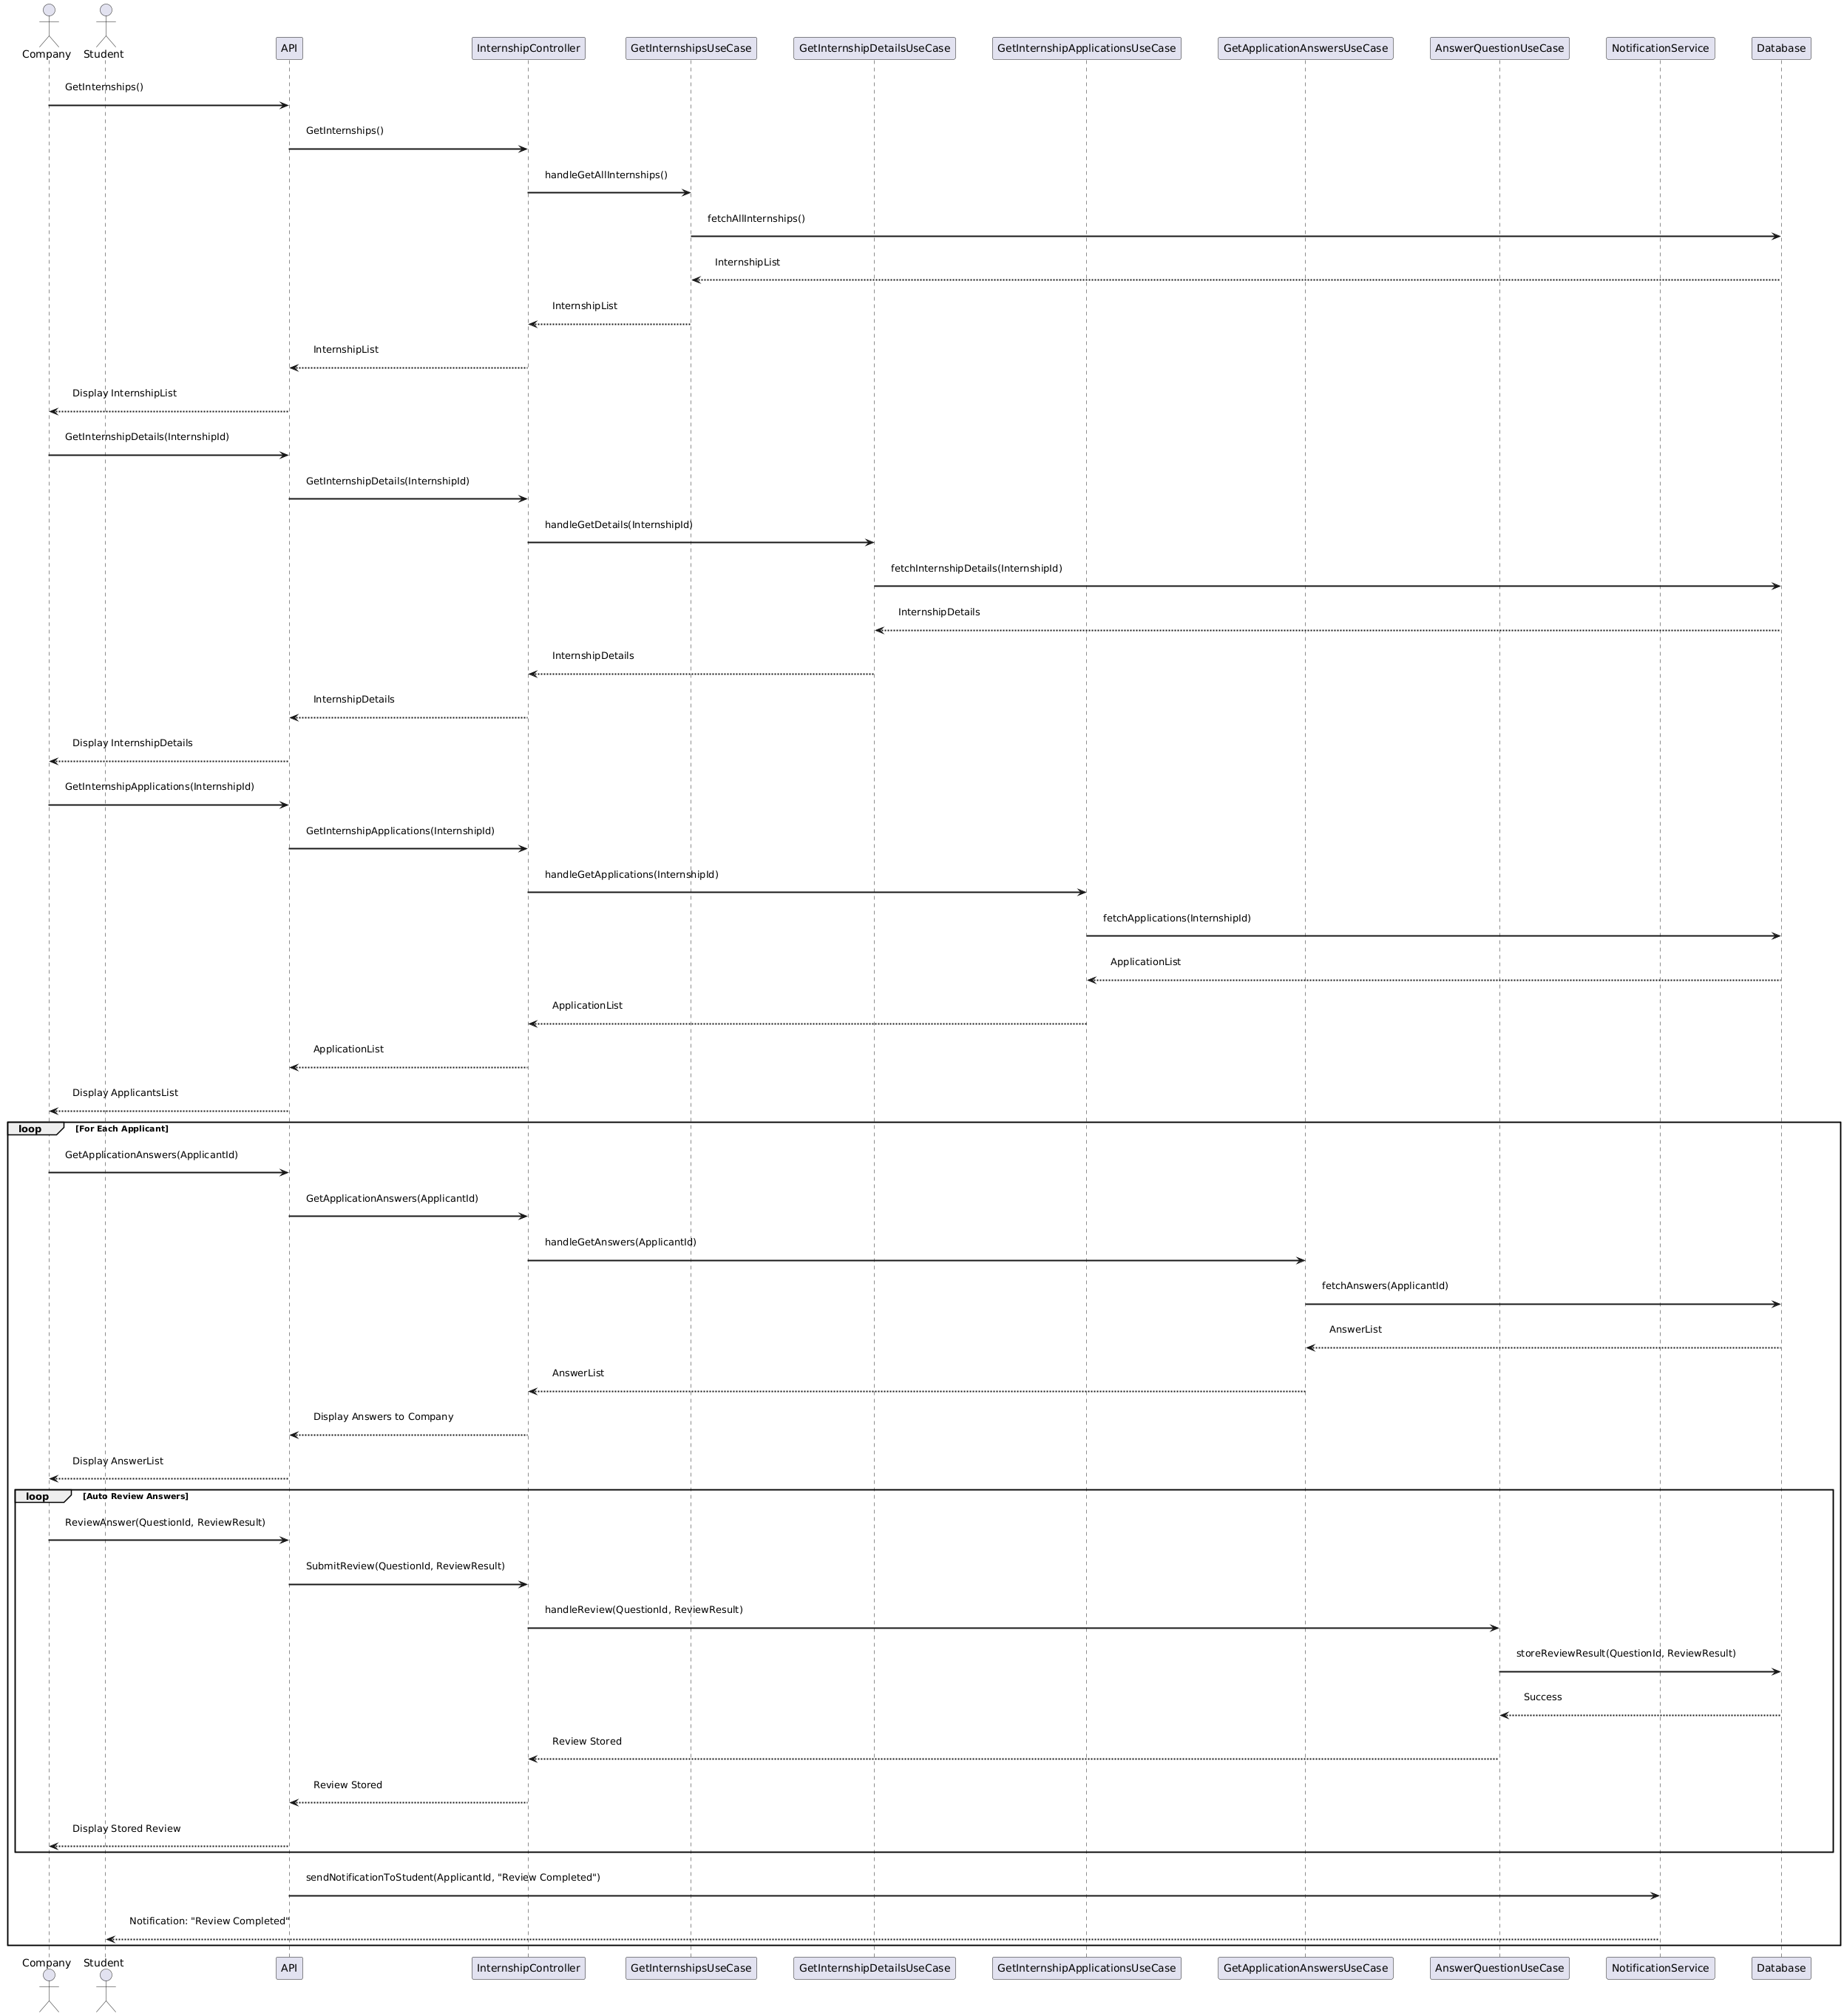
\includegraphics[scale=0.19]{Images/ImagesSequenceDiagram/CompanyReviewsQuestions.png}
    \caption{Company reviews online assessment questions}
\end{figure}

\newpage

\begin{figure}[ht!]
    \centering
    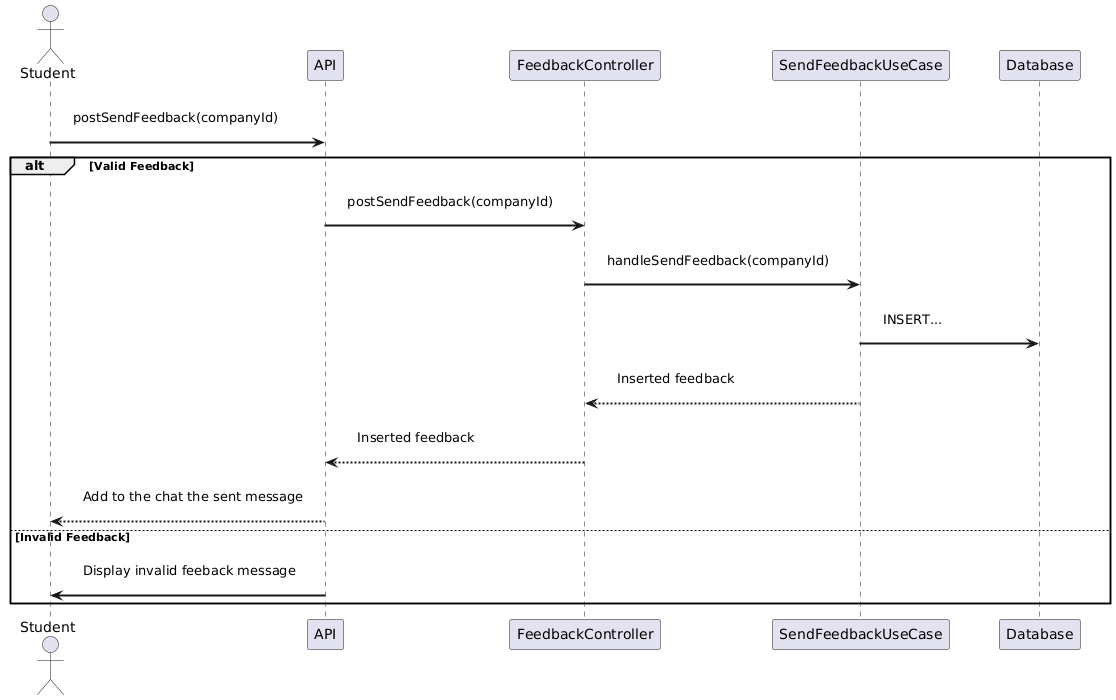
\includegraphics[scale=0.4]{Images/ImagesSequenceDiagram/SendFeebackSD.png}
    \caption{Student(Company) sends feedback to the platform.}
\end{figure}


\newpage

\begin{figure}[ht!]
    \centering
    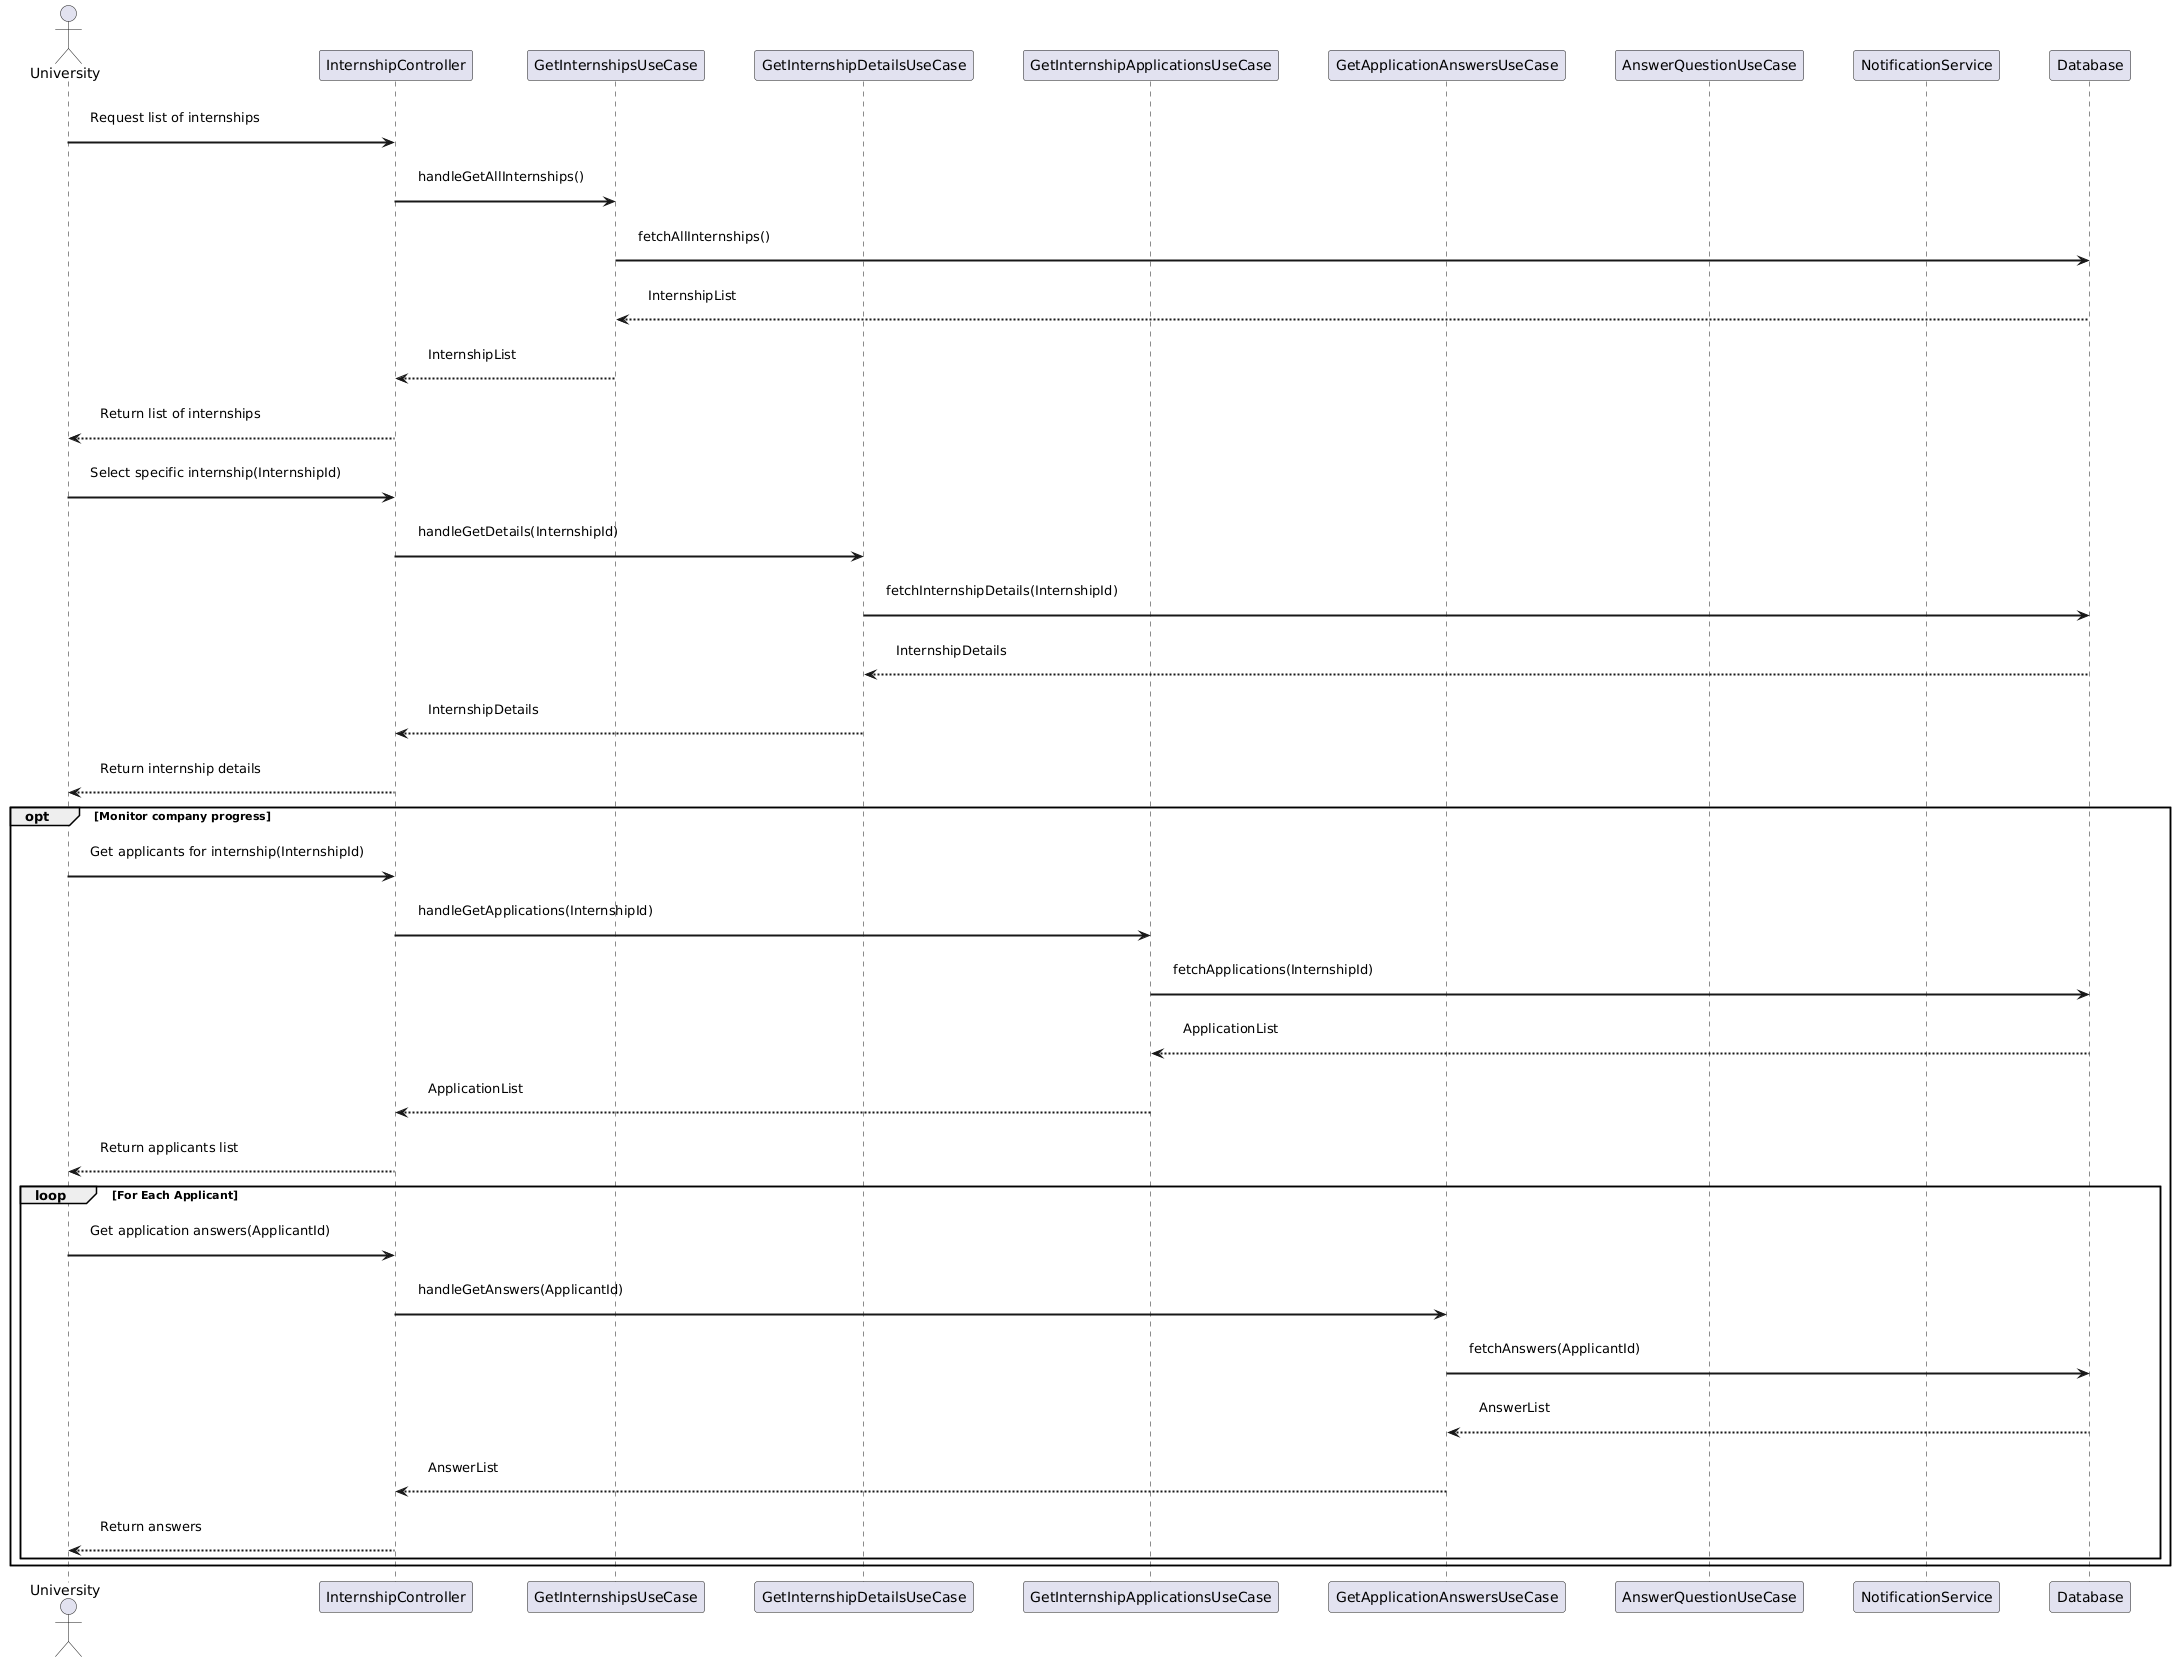
\includegraphics[scale=0.21]{Images/ImagesSequenceDiagram/UniversityMonitorsInternship.png}
    \caption{University monitors the progress of internships}
\end{figure}

\newpage

\section{Component interfaces}

In this section we use the word \textbf{"Dto"} referring to a datatype defined in the backend containing all the required attribute. The input taken from the frontend or the output coming from the backend are mapped into a dto to double check the correctness of the values.

\begin{itemize}
\item \textbf{Authentication}
Handles all processes related to user authentication, such as logging in, logging out, token refreshment, and password management.

\begin{itemize}
    \item \textbf{register(dto: RegisterDto): TokenResponse} – Registers a new user (student, company or university) by saving the provided data and returns a \textit{TokenResponseDto}.
    \item \textbf{login(email: string, password: string): TokenResponseDto} – Authenticates a user (student or company) by validating credentials. If successful, returns a \textit{TokenResponseDto}.
    \item \textbf{logout(): void} – Logs out the user, ending their session.
    \item \textbf{refreshToken(refreshToken: String): TokenResponse} – Extends the session duration by generating a new \textit{authToken} if the refresh token is valid.
    \item \textbf{resetPasswordRequest(email: String): void} – Sends a password reset link to the provided email, allowing users to initiate the password reset process.
    \item \textbf{resetPassword(token: String, newPassword: String): Bool} – Validates the reset token sent to the user's email and updates the password if the token is valid. Returns \textit{true} upon success.
    \item \textbf{verifyEmail(verifyEmail: VerifyEmailDto): VerifyResponse} - verify the email validity.
    \item \textbf{sendVerificationEmail(sendVerify: SendVerificationDto): void} - end the verification email after the registration.
\end{itemize}

\item \textbf{Internship}

\begin{itemize}
\item \textbf{getInternship() : List<InternshipDto> } - Allows platform to retrieve all the internship to fill the homepage.
    \item \textbf{createInternship(companyId: ID, internshipData: Internship): ID} – Allows a company to create a new internship posting, returning the ID of the new internship.
    \item \textbf{applyToInternship(studentId: int, internshiptId: int): ApplicationDto} - Send the student application to a specific internship.
    \iterm \textbf{getInternshipApplicants(internshipId: int, companyId: int): List<StudentDto>} - Retrieves the student that had applied for an internship of a company.
    \item \textbf{updateStatusApplication(applicationId: int, updatedStatus:updatedStatusApplicationDto, companyId: int  ): ApplicationDto} – Updates an existing application changing its status.
    \item \textbf{answerApplicationQuestions(applicationId: int, answer: AnswerQuestionsDto, studentId: int} - Add the student's answers to the application.
    \item \textbf{deleteInternship(internshipId: int): void} – Deletes an internship listing, making it inactive or removing it from the view.
\end{itemize}



\item \textbf{Student}
The Student Controller manages requests related to student profiles, such as updates and viewing application history.

\begin{itemize}
    \item \textbf{getStudent(studentId: int): void} – Get the student profile.
    \item \textbf{updateStudentProfile(studentId: ID, updatedData: UpdateStudentDto): void} – Allows a student to update their profile with new information, such as contact details or academic information.
    \item \textbf{loadCvStudent(dto: LoadCvDto, studentId: int): CvDto}
    \item \textbf{listStudentApplications(studentId: int): List<Application>} – Returns the history of internship applications made by the student.
\end{itemize}

\item \textbf{Match}
The match controller manages finding and retrieving the matches between the company's internship suitable skills and the students' one.
\begin{itemize}

    \item \textbf{GetStudentMatches(studentId: int): List<MatchDto>} - Retrieve the student matches with the intenship of various companies.
    \item \textbf{GetCompanyMathes(companyId: int): List<MatchDto} - Retrieve the company matches between the suitable skills of the students and of their internships.
    \item \textbf{inviteStudent(matchId: int, companyId: int): void} - Company invite a student who is matching with one of its internship.
    \item \textbf{acceptMatch(matchId: int, studentId: int): void} - Student accept one of the invite sent by the company.

\end{itemize}


\item \textbf{Feedback}
The Feedback Controller manages operations for collecting and handling feedback within the system.

\begin{itemize}
    \item \textbf{submitFeedback(userId: ID, internshipId: ID, feedbackData: Feedback): void} – Allows a user (student or company) to submit feedback on an internship or application experience.
    \item \textbf{getFeedbackForInternship(internshipId: ID): List<Feedback>} – Retrieves all feedback associated with a specific internship, useful for administrators to monitor feedback trends.
    \item \textbf{getFeedbackForStudent(studentId: ID): List<Feedback>} – Retrieves feedback given to or by a student, allowing administrators to track individual experiences.
\end{itemize}

\item \textbf{Company}
The Company Controller is responsible for managing company accounts and interaction with internship postings and applications.

\begin{itemize}
    \item \textbf{getProfile(comapanyId: int): CompanyDto} – Creates a new company profile and returns the company ID.
    \item \textbf{updateCompanyProfile(companyId: int, updatedData: CompanyDto): void} – Allows a company to update its profile information, such as contact details or industry.
    \item \textbf{getInternships(companyId: int): List<Internship>} – Lists all internships posted by the company.
    \item \textbf{addInternship(companyId: int, updateData: InternshipDto): void} - Add an internship.
    \item \textbf{updateInternship(companyId: int, internshipId: int, updateData: InternshipUpdateDto): void} - Update a current internship of a company.
    \item \textbf{getQuestions(companyId: int)} - Get the questions created by the companies.
    \item \textbf{addQuestion(companyId: int, updateQuestion: UpdateQuestionDto} - Add a new question.
    \item \textbf{acceptApplication(companyId: int, applicationId: int): void} – Allows a company to accept a student application for an internship.
    \item \textbf{rejectApplication(companyId: int, applicationId: int): void} – Allows a company to reject a student application for an internship.
\end{itemize}

\item \textbf{University}
The university controller is used to manage the university's interactions with students' internships and feedback.
\begin{itemize}
    \item \textbf{getStudentInternshipRecords(studentId: ID): List<Internship>} – Retrieves a list of internships a student has participated in, including completed and current ones.
    \item \textbf{collectFeedback(studentId: ID, internshipId: ID): Feedback} – Collects feedback from students regarding their internship experience for quality assurance and improvement.
    \item \textbf{assignInternshipAdvisor(studentId: ID, advisorId: ID): void} – Assigns an academic advisor to a student's internship to provide guidance and support.
    \item \textbf{listAllFeedback(internshipId: ID): List<Feedback>} – Returns all feedback related to a specific internship to assess overall satisfaction and outcomes.
    \item \textbf{getInternshipApprovalStatus(studentId: ID, internshipId: ID): ApprovalStatus} – Retrieves the current approval status for a student's internship application.
    \item \textbf{updateStudentFeedback(studentId: ID, feedbackId: ID, updatedFeedback: Feedback): void} – Updates feedback provided by a student if changes are needed.
\end{itemize}



\newpage

\end{itemize}


\section{Selected architectural styles and patterns}
\textbf{Monolithic server:} 
We chose a monolithic approach for its simplicity, faster development, and easier management. It minimizes the complexities of inter-service communication and ensures consistent control, which is ideal for smaller teams or projects with limited resources. This approach also offers better performance and simpler security management, making it a practical choice for our project’s scope

\textbf{Fat client:}
Fat clients allow offering a wide variety of functionalities independent from the central server, as well as to move part of the business logic off of the server and into the clients. The main advantages it offers are greater decoupling of frontend and backend as well as a better interactive experience, especially in conditions where the client is on an unstable network. Additionally, with the adoption of a single-page applications, there are many cross-platform frameworks which allow to reuse code partially or entirely on multiple platforms. The single-page web application can also be served by a dedicated static web server, as all its interactivity is implemented client-side, further reducing the burden on the server by delegating its serving to a CDN, which is highly optimized for
this specific use case.

\textbf{REST API:}
An architectural style defined on top of HTTP centered around the definition of a standardized set of stateless operations. Its main advantages are its simplicity, its use of widely adopted standards which facilitate adoption, and its ease of scalability given by its stateless nature. It allows to have a single API interface against which a heterogeneous set of clients can make requests.

\textbf{Component-based architecture:}
In the frontend, we have focused on a component-based architecture. This approach structures the application as a collection of reusable and self-contained components, each managing its logic, rendering, and state. By adopting this architecture, we ensure that the code is modular, making it easier to maintain, update. Reusability is a key advantage, as components can be composed and reused across different sections of the app, leading to more efficient development and consistent user interfaces.


\section{Other design decisions}

\textbf{Relational DBMS}: 
We chose to integrate a Database Management System (DBMS) into our project to ensure efficient data management, storage, and retrieval. A DBMS provides a structured and scalable way to handle large volumes of data while maintaining data integrity, consistency, and security. It allows for multi-user access, concurrent data manipulation, and facilitates complex queries that enhance the project's functionality and performance. The choice of a DBMS also supports data backup and recovery, reducing the risk of data loss and ensuring system reliability. Overall, it is an essential component for building a robust, reliable, and scalable solution
